% Generated by Sphinx.
\def\sphinxdocclass{report}
\documentclass[letterpaper,10pt,english]{sphinxmanual}
\usepackage[utf8]{inputenc}
\DeclareUnicodeCharacter{00A0}{\nobreakspace}
\usepackage{cmap}
\usepackage[T1]{fontenc}
\usepackage{babel}
\usepackage{times}
\usepackage[Bjarne]{fncychap}
\usepackage{longtable}
\usepackage{sphinx}
\usepackage{multirow}

\addto\captionsenglish{\renewcommand{\figurename}{Fig. }}
\addto\captionsenglish{\renewcommand{\tablename}{Table }}
\floatname{literal-block}{Listing }




%%%%%%%%%%%%%%%%%%%%%%%%%%%%%%%%%%%%%
%%% MANUALLY ADDED/EDITED
\newcommand{\disclaimer}{%
\thispagestyle{empty}% no number of this page
\vglue5\baselineskip
\begin{center}
{\bf DISCLAIMER}
\end{center}
\noindent
This document was prepared as an account of work sponsored by an agency of 
the United States government. Neither the United States government nor 
Lawrence Livermore National Security, LLC, nor Southern Methodist
University, nor any of their employees makes any warranty, expressed
or implied, or assumes any legal liability or responsibility for the
accuracy, completeness, or usefulness of any information, apparatus,
product, or process disclosed, or represents that its use would not
infringe privately owned rights.  Reference herein to any specific
commercial product, process, or service by trade name, trademark,
manufacturer, or otherwise does not necessarily constitute or imply
its endorsement, recommendation, or favoring by the United States
government, Lawrence Livermore National Security, LLC, or Southern
Methodist University. The views and opinions of authors expressed
herein do not necessarily state or reflect those of the United States
government, Lawrence Livermore National Security, LLC, or Southern
Methodist University, and shall not be used for advertising or product
endorsement purposes.

\vskip2\baselineskip
%\noindent This work was performed under the auspices of the U.S. Department of Energy by Lawrence 
%Livermore National Laboratory under Contract DE-AC52-07NA27344.
\vfill
\begin{center}
Approved for public release; further dissemination unlimited
\end{center}
\clearpage
}

\title{Example Programs for ARKode}
\author{Daniel R. Reynolds\\
  {\em Department of Mathematics}\\
  {\em Southern Methodist University}
}
\date{
  \today
  \vfill
  {\centerline{\includegraphics[width=0.5\textwidth]{doc_logo_blue.pdf}}}
  \vfill
}
\release{3.0.2}
%%%%%%%%%%%%%%%%%%%%%%%%%%%%%%%%%%%%%



\newcommand{\sphinxlogo}{}
\renewcommand{\releasename}{Release}
\makeindex

\makeatletter
\def\PYG@reset{\let\PYG@it=\relax \let\PYG@bf=\relax%
    \let\PYG@ul=\relax \let\PYG@tc=\relax%
    \let\PYG@bc=\relax \let\PYG@ff=\relax}
\def\PYG@tok#1{\csname PYG@tok@#1\endcsname}
\def\PYG@toks#1+{\ifx\relax#1\empty\else%
    \PYG@tok{#1}\expandafter\PYG@toks\fi}
\def\PYG@do#1{\PYG@bc{\PYG@tc{\PYG@ul{%
    \PYG@it{\PYG@bf{\PYG@ff{#1}}}}}}}
\def\PYG#1#2{\PYG@reset\PYG@toks#1+\relax+\PYG@do{#2}}

\expandafter\def\csname PYG@tok@gd\endcsname{\def\PYG@tc##1{\textcolor[rgb]{0.63,0.00,0.00}{##1}}}
\expandafter\def\csname PYG@tok@gu\endcsname{\let\PYG@bf=\textbf\def\PYG@tc##1{\textcolor[rgb]{0.50,0.00,0.50}{##1}}}
\expandafter\def\csname PYG@tok@gt\endcsname{\def\PYG@tc##1{\textcolor[rgb]{0.00,0.27,0.87}{##1}}}
\expandafter\def\csname PYG@tok@gs\endcsname{\let\PYG@bf=\textbf}
\expandafter\def\csname PYG@tok@gr\endcsname{\def\PYG@tc##1{\textcolor[rgb]{1.00,0.00,0.00}{##1}}}
\expandafter\def\csname PYG@tok@cm\endcsname{\let\PYG@it=\textit\def\PYG@tc##1{\textcolor[rgb]{0.25,0.50,0.56}{##1}}}
\expandafter\def\csname PYG@tok@vg\endcsname{\def\PYG@tc##1{\textcolor[rgb]{0.73,0.38,0.84}{##1}}}
\expandafter\def\csname PYG@tok@vi\endcsname{\def\PYG@tc##1{\textcolor[rgb]{0.73,0.38,0.84}{##1}}}
\expandafter\def\csname PYG@tok@vm\endcsname{\def\PYG@tc##1{\textcolor[rgb]{0.73,0.38,0.84}{##1}}}
\expandafter\def\csname PYG@tok@mh\endcsname{\def\PYG@tc##1{\textcolor[rgb]{0.13,0.50,0.31}{##1}}}
\expandafter\def\csname PYG@tok@cs\endcsname{\def\PYG@tc##1{\textcolor[rgb]{0.25,0.50,0.56}{##1}}\def\PYG@bc##1{\setlength{\fboxsep}{0pt}\colorbox[rgb]{1.00,0.94,0.94}{\strut ##1}}}
\expandafter\def\csname PYG@tok@ge\endcsname{\let\PYG@it=\textit}
\expandafter\def\csname PYG@tok@vc\endcsname{\def\PYG@tc##1{\textcolor[rgb]{0.73,0.38,0.84}{##1}}}
\expandafter\def\csname PYG@tok@il\endcsname{\def\PYG@tc##1{\textcolor[rgb]{0.13,0.50,0.31}{##1}}}
\expandafter\def\csname PYG@tok@go\endcsname{\def\PYG@tc##1{\textcolor[rgb]{0.20,0.20,0.20}{##1}}}
\expandafter\def\csname PYG@tok@cp\endcsname{\def\PYG@tc##1{\textcolor[rgb]{0.00,0.44,0.13}{##1}}}
\expandafter\def\csname PYG@tok@gi\endcsname{\def\PYG@tc##1{\textcolor[rgb]{0.00,0.63,0.00}{##1}}}
\expandafter\def\csname PYG@tok@gh\endcsname{\let\PYG@bf=\textbf\def\PYG@tc##1{\textcolor[rgb]{0.00,0.00,0.50}{##1}}}
\expandafter\def\csname PYG@tok@ni\endcsname{\let\PYG@bf=\textbf\def\PYG@tc##1{\textcolor[rgb]{0.84,0.33,0.22}{##1}}}
\expandafter\def\csname PYG@tok@nl\endcsname{\let\PYG@bf=\textbf\def\PYG@tc##1{\textcolor[rgb]{0.00,0.13,0.44}{##1}}}
\expandafter\def\csname PYG@tok@nn\endcsname{\let\PYG@bf=\textbf\def\PYG@tc##1{\textcolor[rgb]{0.05,0.52,0.71}{##1}}}
\expandafter\def\csname PYG@tok@no\endcsname{\def\PYG@tc##1{\textcolor[rgb]{0.38,0.68,0.84}{##1}}}
\expandafter\def\csname PYG@tok@na\endcsname{\def\PYG@tc##1{\textcolor[rgb]{0.25,0.44,0.63}{##1}}}
\expandafter\def\csname PYG@tok@nb\endcsname{\def\PYG@tc##1{\textcolor[rgb]{0.00,0.44,0.13}{##1}}}
\expandafter\def\csname PYG@tok@nc\endcsname{\let\PYG@bf=\textbf\def\PYG@tc##1{\textcolor[rgb]{0.05,0.52,0.71}{##1}}}
\expandafter\def\csname PYG@tok@nd\endcsname{\let\PYG@bf=\textbf\def\PYG@tc##1{\textcolor[rgb]{0.33,0.33,0.33}{##1}}}
\expandafter\def\csname PYG@tok@ne\endcsname{\def\PYG@tc##1{\textcolor[rgb]{0.00,0.44,0.13}{##1}}}
\expandafter\def\csname PYG@tok@nf\endcsname{\def\PYG@tc##1{\textcolor[rgb]{0.02,0.16,0.49}{##1}}}
\expandafter\def\csname PYG@tok@si\endcsname{\let\PYG@it=\textit\def\PYG@tc##1{\textcolor[rgb]{0.44,0.63,0.82}{##1}}}
\expandafter\def\csname PYG@tok@s2\endcsname{\def\PYG@tc##1{\textcolor[rgb]{0.25,0.44,0.63}{##1}}}
\expandafter\def\csname PYG@tok@nt\endcsname{\let\PYG@bf=\textbf\def\PYG@tc##1{\textcolor[rgb]{0.02,0.16,0.45}{##1}}}
\expandafter\def\csname PYG@tok@nv\endcsname{\def\PYG@tc##1{\textcolor[rgb]{0.73,0.38,0.84}{##1}}}
\expandafter\def\csname PYG@tok@s1\endcsname{\def\PYG@tc##1{\textcolor[rgb]{0.25,0.44,0.63}{##1}}}
\expandafter\def\csname PYG@tok@dl\endcsname{\def\PYG@tc##1{\textcolor[rgb]{0.25,0.44,0.63}{##1}}}
\expandafter\def\csname PYG@tok@ch\endcsname{\let\PYG@it=\textit\def\PYG@tc##1{\textcolor[rgb]{0.25,0.50,0.56}{##1}}}
\expandafter\def\csname PYG@tok@m\endcsname{\def\PYG@tc##1{\textcolor[rgb]{0.13,0.50,0.31}{##1}}}
\expandafter\def\csname PYG@tok@gp\endcsname{\let\PYG@bf=\textbf\def\PYG@tc##1{\textcolor[rgb]{0.78,0.36,0.04}{##1}}}
\expandafter\def\csname PYG@tok@sh\endcsname{\def\PYG@tc##1{\textcolor[rgb]{0.25,0.44,0.63}{##1}}}
\expandafter\def\csname PYG@tok@ow\endcsname{\let\PYG@bf=\textbf\def\PYG@tc##1{\textcolor[rgb]{0.00,0.44,0.13}{##1}}}
\expandafter\def\csname PYG@tok@sx\endcsname{\def\PYG@tc##1{\textcolor[rgb]{0.78,0.36,0.04}{##1}}}
\expandafter\def\csname PYG@tok@bp\endcsname{\def\PYG@tc##1{\textcolor[rgb]{0.00,0.44,0.13}{##1}}}
\expandafter\def\csname PYG@tok@c1\endcsname{\let\PYG@it=\textit\def\PYG@tc##1{\textcolor[rgb]{0.25,0.50,0.56}{##1}}}
\expandafter\def\csname PYG@tok@fm\endcsname{\def\PYG@tc##1{\textcolor[rgb]{0.02,0.16,0.49}{##1}}}
\expandafter\def\csname PYG@tok@o\endcsname{\def\PYG@tc##1{\textcolor[rgb]{0.40,0.40,0.40}{##1}}}
\expandafter\def\csname PYG@tok@kc\endcsname{\let\PYG@bf=\textbf\def\PYG@tc##1{\textcolor[rgb]{0.00,0.44,0.13}{##1}}}
\expandafter\def\csname PYG@tok@c\endcsname{\let\PYG@it=\textit\def\PYG@tc##1{\textcolor[rgb]{0.25,0.50,0.56}{##1}}}
\expandafter\def\csname PYG@tok@mf\endcsname{\def\PYG@tc##1{\textcolor[rgb]{0.13,0.50,0.31}{##1}}}
\expandafter\def\csname PYG@tok@err\endcsname{\def\PYG@bc##1{\setlength{\fboxsep}{0pt}\fcolorbox[rgb]{1.00,0.00,0.00}{1,1,1}{\strut ##1}}}
\expandafter\def\csname PYG@tok@mb\endcsname{\def\PYG@tc##1{\textcolor[rgb]{0.13,0.50,0.31}{##1}}}
\expandafter\def\csname PYG@tok@ss\endcsname{\def\PYG@tc##1{\textcolor[rgb]{0.32,0.47,0.09}{##1}}}
\expandafter\def\csname PYG@tok@sr\endcsname{\def\PYG@tc##1{\textcolor[rgb]{0.14,0.33,0.53}{##1}}}
\expandafter\def\csname PYG@tok@mo\endcsname{\def\PYG@tc##1{\textcolor[rgb]{0.13,0.50,0.31}{##1}}}
\expandafter\def\csname PYG@tok@kd\endcsname{\let\PYG@bf=\textbf\def\PYG@tc##1{\textcolor[rgb]{0.00,0.44,0.13}{##1}}}
\expandafter\def\csname PYG@tok@mi\endcsname{\def\PYG@tc##1{\textcolor[rgb]{0.13,0.50,0.31}{##1}}}
\expandafter\def\csname PYG@tok@kn\endcsname{\let\PYG@bf=\textbf\def\PYG@tc##1{\textcolor[rgb]{0.00,0.44,0.13}{##1}}}
\expandafter\def\csname PYG@tok@cpf\endcsname{\let\PYG@it=\textit\def\PYG@tc##1{\textcolor[rgb]{0.25,0.50,0.56}{##1}}}
\expandafter\def\csname PYG@tok@kr\endcsname{\let\PYG@bf=\textbf\def\PYG@tc##1{\textcolor[rgb]{0.00,0.44,0.13}{##1}}}
\expandafter\def\csname PYG@tok@s\endcsname{\def\PYG@tc##1{\textcolor[rgb]{0.25,0.44,0.63}{##1}}}
\expandafter\def\csname PYG@tok@kp\endcsname{\def\PYG@tc##1{\textcolor[rgb]{0.00,0.44,0.13}{##1}}}
\expandafter\def\csname PYG@tok@w\endcsname{\def\PYG@tc##1{\textcolor[rgb]{0.73,0.73,0.73}{##1}}}
\expandafter\def\csname PYG@tok@kt\endcsname{\def\PYG@tc##1{\textcolor[rgb]{0.56,0.13,0.00}{##1}}}
\expandafter\def\csname PYG@tok@sc\endcsname{\def\PYG@tc##1{\textcolor[rgb]{0.25,0.44,0.63}{##1}}}
\expandafter\def\csname PYG@tok@sb\endcsname{\def\PYG@tc##1{\textcolor[rgb]{0.25,0.44,0.63}{##1}}}
\expandafter\def\csname PYG@tok@sa\endcsname{\def\PYG@tc##1{\textcolor[rgb]{0.25,0.44,0.63}{##1}}}
\expandafter\def\csname PYG@tok@k\endcsname{\let\PYG@bf=\textbf\def\PYG@tc##1{\textcolor[rgb]{0.00,0.44,0.13}{##1}}}
\expandafter\def\csname PYG@tok@se\endcsname{\let\PYG@bf=\textbf\def\PYG@tc##1{\textcolor[rgb]{0.25,0.44,0.63}{##1}}}
\expandafter\def\csname PYG@tok@sd\endcsname{\let\PYG@it=\textit\def\PYG@tc##1{\textcolor[rgb]{0.25,0.44,0.63}{##1}}}

\def\PYGZbs{\char`\\}
\def\PYGZus{\char`\_}
\def\PYGZob{\char`\{}
\def\PYGZcb{\char`\}}
\def\PYGZca{\char`\^}
\def\PYGZam{\char`\&}
\def\PYGZlt{\char`\<}
\def\PYGZgt{\char`\>}
\def\PYGZsh{\char`\#}
\def\PYGZpc{\char`\%}
\def\PYGZdl{\char`\$}
\def\PYGZhy{\char`\-}
\def\PYGZsq{\char`\'}
\def\PYGZdq{\char`\"}
\def\PYGZti{\char`\~}
% for compatibility with earlier versions
\def\PYGZat{@}
\def\PYGZlb{[}
\def\PYGZrb{]}
\makeatother

\renewcommand\PYGZsq{\textquotesingle}

\begin{document}

\maketitle
\tableofcontents
\phantomsection\label{index::doc}


This is the documentation for the ARKode examples.  ARKode is an
adaptive step time integration package for stiff, nonstiff and
multi-rate systems of ordinary differential equations (ODEs).
The ARKode solver is a component of the \href{https://computation.llnl.gov/casc/sundials/main.html}{SUNDIALS} suite of
nonlinear and differential/algebraic equation solvers. It is designed
to have a similar user experience to the \href{https://computation.llnl.gov/casc/sundials/description/description.html\#descr\_cvode}{CVODE}
solver, with user modes to allow adaptive integration to specified
output times, return after each internal step and root-finding
capabilities, for calculations both in serial and parallel (via
MPI). The default integration and solver options should apply to most
users, though complete control over all internal parameters and time
adaptivity algorithms is enabled through optional interface routines.

ARKode is developed by \href{http://www.smu.edu}{Southern Methodist University}, with support by the \href{http://www.doe.gov}{US Department of Energy} through the \href{http://www.fastmath-scidac.org/}{FASTMath} SciDAC Institute, under subcontract
B598130 from \href{http://www.llnl.gov}{Lawrence Livermore National Laboratory}.

Along with the ARKode solver, we have created a suite of example
problems demonstrating its usage on applications written in C, C++ and
Fortran 77 and Fortran 90.  These examples demonstrate a large variety
of ARKode solver options, including explicit, implicit and ImEx
solvers, root-finding, Newton and fixed-point nonlinear solvers,
direct and iterative linear solvers, adaptive resize capabilities, and
the Fortran solver interface.  While these examples are not an
exhaustive set of all possible usage scenarios, they are designed to
show a variety of exemplars, and can be used as templates for new
problems using ARKode's solvers.  Further information on the ARKode
package itself may be found in the accompanying ARKode user guide
\phantomsection\label{index:id1}{\hyperref[References:r2018]{\emph{{[}R2018{]}}}}.

The following tables summarize the salient features of each of the
example problems in this document.  Each example is designed to be
relatively self-contained, so that you need only study and/or emulate
the problem that is most closely related to your own.  We group these
examples according to programming language (C, C++, Fortran 77,
Fortran 90).

ARKode example problems written in C are summarized in the table
below, and are further described in the chapters {\hyperref[c_serial:serial-c]{\emph{\DUspan{}{Serial C example problems}}}},
{\hyperref[c_openmp:openmp-c]{\emph{\DUspan{}{OpenMP C example problems}}}}, {\hyperref[c_parallel:parallel-c]{\emph{\DUspan{}{Parallel C example problems}}}} and {\hyperref[c_parhyp:parhyp-c]{\emph{\DUspan{}{Parallel Hypre example problems}}}}.

\begin{tabulary}{\linewidth}{|L|L|L|L|L|L|}
\hline
\textsf{\relax 
Problem
} & \textsf{\relax 
Integrator
} & \textsf{\relax 
Nonlinear
} & \textsf{\relax 
Linear
} & \textsf{\relax 
Size
} & \textsf{\relax 
Extras
}\\
\hline
{\hyperref[c_serial:ark-analytic]{\emph{\DUspan{}{ark\_analytic}}}}
 & 
DIRK
 & 
Newton
 & 
Dense
 & 
1
 & \\
\hline
{\hyperref[c_serial:ark-analytic-nonlin]{\emph{\DUspan{}{ark\_analytic\_nonlin}}}}
 & 
ERK
 & 
N.A.
 & 
N.A.
 & 
1
 & 
ERKStep timestepping module
\\
\hline
{\hyperref[c_serial:ark-brusselator]{\emph{\DUspan{}{ark\_brusselator}}}}
 & 
DIRK
 & 
Newton
 & 
Dense
 & 
3
 & \\
\hline
{\hyperref[c_serial:ark-brusselator-fp]{\emph{\DUspan{}{ark\_brusselator\_fp}}}}
 & 
ARK
 & 
Fixed-point
 & 
N.A.
 & 
3
 & \\
\hline
{\hyperref[c_serial:ark-robertson]{\emph{\DUspan{}{ark\_robertson}}}}
 & 
DIRK
 & 
Newton
 & 
Dense
 & 
3
 & \\
\hline
{\hyperref[c_serial:ark-robertson-root]{\emph{\DUspan{}{ark\_robertson\_root}}}}
 & 
DIRK
 & 
Newton
 & 
Dense
 & 
3
 & 
rootfinding
\\
\hline
{\hyperref[c_serial:ark-brusselator1d]{\emph{\DUspan{}{ark\_brusselator1D}}}}
 & 
DIRK
 & 
Newton
 & 
Band
 & 
3N
 & \\
\hline
{\hyperref[c_openmp:ark-brusselator1d-omp]{\emph{\DUspan{}{ark\_brusselator1D\_omp}}}}
 & 
DIRK
 & 
Newton
 & 
Band
 & 
3N
 & 
OpenMP-enabled
\\
\hline
{\hyperref[c_serial:ark-brusselator1d-klu]{\emph{\DUspan{}{ark\_brusselator1D\_klu}}}}
 & 
DIRK
 & 
Newton
 & 
KLU
 & 
3N
 & 
sparse matrices
\\
\hline
{\hyperref[c_serial:ark-brusselator1d-fem-slu]{\emph{\DUspan{}{ark\_brusselator1D\_FEM\_slu}}}}
 & 
DIRK
 & 
Newton
 & 
SuperLU\_MT
 & 
3N
 & 
finite-element, \(M\ne I\), sparse matrices
\\
\hline
{\hyperref[c_serial:ark-heat1d]{\emph{\DUspan{}{ark\_heat1D}}}}
 & 
DIRK
 & 
Newton
 & 
PCG
 & 
N
 & \\
\hline
{\hyperref[c_serial:ark-heat1d-adapt]{\emph{\DUspan{}{ark\_heat1D\_adapt}}}}
 & 
DIRK
 & 
Newton
 & 
PCG
 & 
(dynamic)
 & 
adaptive vector resizing
\\
\hline
{\hyperref[c_serial:ark-krylovdemo-prec]{\emph{\DUspan{}{ark\_KrylovDemo\_prec}}}}
 & 
DIRK
 & 
Newton
 & 
SPGMR
 & 
216
 & 
multiple preconditioners
\\
\hline
{\hyperref[c_parallel:ark-diurnal-kry-bbd-p]{\emph{\DUspan{}{ark\_diurnal\_kry\_bbd\_p}}}}
 & 
DIRK
 & 
Newton
 & 
SPGMR
 & 
200
 & 
parallel, BBD preconditioner
\\
\hline
{\hyperref[c_parallel:ark-diurnal-kry-p]{\emph{\DUspan{}{ark\_diurnal\_kry\_p}}}}
 & 
DIRK
 & 
Newton
 & 
SPGMR
 & 
200
 & 
parallel, block-diagonal precond.
\\
\hline
{\hyperref[c_parhyp:ark-diurnal-kry-ph]{\emph{\DUspan{}{ark\_diurnal\_kry\_ph}}}}
 & 
DIRK
 & 
Newton
 & 
SPGMR
 & 
200
 & 
HYPRE parallel vector
\\
\hline\end{tabulary}


ARKode example problems written in C++ are summarized in the table
below, and are further described in the chapters {\hyperref[cpp_serial:serial-cpp]{\emph{\DUspan{}{Serial C++ example problems}}}} and
{\hyperref[cpp_parallel:parallel-cpp]{\emph{\DUspan{}{Parallel C++ example problems}}}}.

\begin{tabulary}{\linewidth}{|L|L|L|L|L|L|}
\hline
\textsf{\relax 
Problem
} & \textsf{\relax 
Integrator
} & \textsf{\relax 
Nonlinear
} & \textsf{\relax 
Linear
} & \textsf{\relax 
Size
} & \textsf{\relax 
Extras
}\\
\hline
{\hyperref[cpp_serial:ark-analytic-sys]{\emph{\DUspan{}{ark\_analytic\_sys}}}}
 & 
DIRK
 & 
Newton
 & 
Dense
 & 
3
 & \\
\hline
{\hyperref[cpp_parallel:ark-heat2d]{\emph{\DUspan{}{ark\_heat2D}}}}
 & 
DIRK
 & 
Newton
 & 
PCG
 & 
\(nx*ny\)
 & 
parallel
\\
\hline\end{tabulary}


ARKode example problems written in Fortran 77 are summarized in the table
below, and are further described in the chapters {\hyperref[f77_serial:serial-f77]{\emph{\DUspan{}{Serial Fortran 77 example problems}}}} and
{\hyperref[f77_parallel:parallel-f77]{\emph{\DUspan{}{Parallel Fortran 77 example problems}}}}.

\begin{tabulary}{\linewidth}{|L|L|L|L|L|L|}
\hline
\textsf{\relax 
Problem
} & \textsf{\relax 
Integrator
} & \textsf{\relax 
Nonlinear
} & \textsf{\relax 
Linear
} & \textsf{\relax 
Size
} & \textsf{\relax 
Extras
}\\
\hline
{\hyperref[f77_serial:fark-diurnal-kry-bp]{\emph{\DUspan{}{fark\_diurnal\_kry\_bp}}}}
 & 
DIRK
 & 
Newton
 & 
SPGMR
 & 
10
 & 
banded preconditioner
\\
\hline
{\hyperref[f77_serial:fark-roberts-dnsl]{\emph{\DUspan{}{fark\_roberts\_dnsL}}}}
 & 
DIRK
 & 
Newton
 & 
Dense
 & 
3
 & 
LAPACK dense solver, rootfinding
\\
\hline
{\hyperref[f77_parallel:fark-diag-kry-bbd-p]{\emph{\DUspan{}{fark\_diag\_kry\_bbd\_p}}}}
 & 
DIRK
 & 
Newton
 & 
SPGMR
 & 
10*NProcs
 & 
parallel BBD preconditioner
\\
\hline
{\hyperref[f77_parallel:fark-diag-non-p]{\emph{\DUspan{}{fark\_diag\_non\_p}}}}
 & 
ERK
 & 
N.A.
 & 
N.A.
 & 
10*NProcs
 & 
parallel
\\
\hline\end{tabulary}


ARKode example problems written in Fortran 90 are summarized in the table
below, and are further described in the chapters {\hyperref[f90_serial:serial-f90]{\emph{\DUspan{}{Serial Fortran 90 example problems}}}} and
{\hyperref[f90_parallel:parallel-f90]{\emph{\DUspan{}{Parallel Fortran 90 example problems}}}}.

\begin{tabulary}{\linewidth}{|L|L|L|L|L|L|}
\hline
\textsf{\relax 
Problem
} & \textsf{\relax 
Integrator
} & \textsf{\relax 
Nonlinear
} & \textsf{\relax 
Linear
} & \textsf{\relax 
Size
} & \textsf{\relax 
Extras
}\\
\hline
{\hyperref[f90_serial:ark-bruss]{\emph{\DUspan{}{ark\_bruss}}}}
 & 
ARK
 & 
Newton
 & 
Dense
 & 
3
 & \\
\hline
{\hyperref[f90_serial:ark-bruss1d-fem-klu]{\emph{\DUspan{}{ark\_bruss1D\_FEM\_klu}}}}
 & 
DIRK
 & 
Newton
 & 
KLU
 & 
3N
 & 
finite-element, \(M\ne I\), sparse matrices
\\
\hline
{\hyperref[f90_parallel:fark-heat2d]{\emph{\DUspan{}{fark\_heat2D}}}}
 & 
DIRK
 & 
Newton
 & 
PCG
 & 
\(nx*ny\)
 & 
parallel
\\
\hline\end{tabulary}



\chapter{Serial C example problems}
\label{c_serial:serial-c}\label{c_serial::doc}\label{c_serial:arkode-example-documentation}\label{c_serial:serial-c-example-problems}

\section{ark\_analytic}
\label{c_serial:ark-analytic}\label{c_serial:id1}
This is a very simple C example showing how to use the ARKode solver
interface.

The problem is that of a scalar-valued initial value problem (IVP)
that is linear in the dependent variable \(y\), but nonlinear in
the independent variable \(t\):
\begin{gather}
\begin{split}\frac{dy}{dt} = \lambda y + \frac{1}{1+t^2} - \lambda \arctan(t),\end{split}\notag
\end{gather}
where \(0\le t\le 10\) and \(y(0)=0\).  The stiffness of the
problem may be tuned via the parameter \(\lambda\).  The value of
\(\lambda\) must be negative to result in a well-posed problem;
for values with magnitude larger than 100 or so the problem becomes
quite stiff.  Here, we choose \(\lambda=-100\).  After each unit
time interval, the solution is output to the screen.


\subsection{Numerical method}
\label{c_serial:numerical-method}
The example routine solves this problem using a diagonally-implicit
Runge-Kutta method.  Each stage is solved using the built-in modified
Newton iteration, but since the ODE is linear in \(y\) these
should only require a single iteration per stage.  Internally, Newton
will use the SUNLINSOL\_DENSE linear solver via the ARKDLS interface,
which in the case of this scalar-valued problem is just division.  The
example file contains functions to evaluate both \(f(t,y)\) and
\(J(t,y)=\lambda\).

We specify the relative and absolute tolerances, \(rtol=10^{-6}\)
and \(atol=10^{-10}\), respectively.  Aside from these choices,
this problem uses only the default ARKode solver parameters.


\subsection{Solutions}
\label{c_serial:solutions}
This problem is included both as a simple example, but also because it
has an analytical solution, \(y(t) = \arctan(t)\).  As seen in the
plots below, the computed solution tracks the analytical solution
quite well (left), and results in errors below those specified by the input
error tolerances (right).

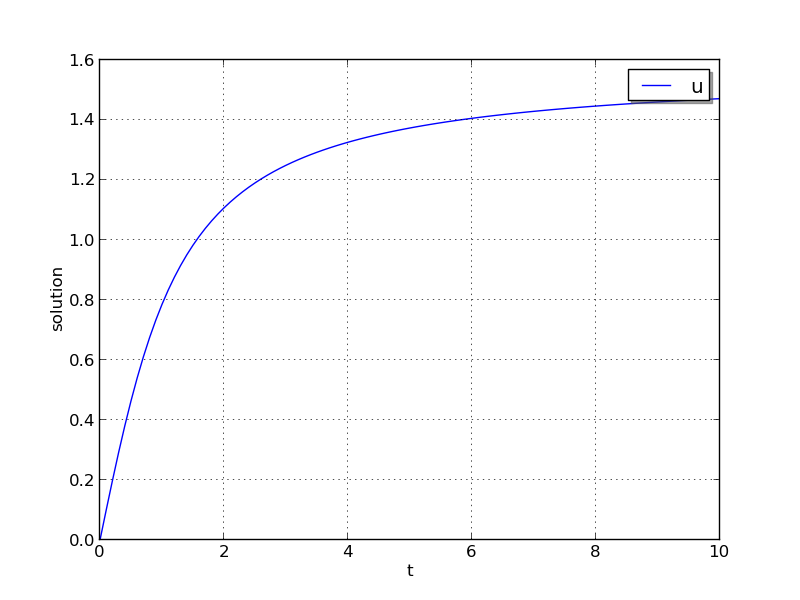
\includegraphics[width=0.450\linewidth]{plot-ark_analytic.png}

\includegraphics[width=0.450\linewidth]{plot-ark_analytic_error.png}


\section{ark\_analytic\_nonlin}
\label{c_serial:id2}\label{c_serial:ark-analytic-nonlin}
This example problem is only marginally more difficult than the
preceding problem, in that the ODE right-hand side function is
nonlinear in the solution \(y\).  While the implicit solver from
the preceding problem would also work on this example, because it is
not stiff we use this to demonstrate how to use ARKode's explicit
solver interface.  Although both the ARKStep and ERKStep time stepping
modules are appropriate in this scenario, we use the ERKStep module
here.

The ODE problem is
\begin{gather}
\begin{split}\frac{dy}{dt} = (t+1) e^{-y},\end{split}\notag
\end{gather}
for the interval \(t \in [0.0, 10.0]\), with initial condition
\(y(0)=0\).  This has analytical solution \(y(t) =
\log\left(\frac{t^2}{2} + t + 1\right)\).


\subsection{Numerical method}
\label{c_serial:id3}
This program solves the problem with the default ERK method.  Output
is printed every 1.0 units of time (10 total).
Run statistics (optional outputs) are printed at the end.


\subsection{Solutions}
\label{c_serial:id4}
As seen in the plots below, the computed solution tracks the
analytical solution quite well (left), and results in errors
comparable with those specified by the requested error tolerances
(right).

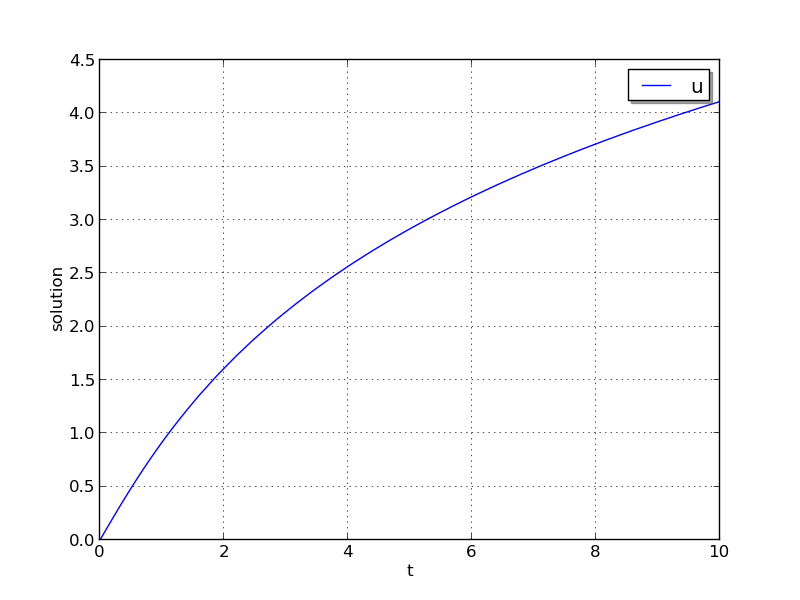
\includegraphics[width=0.450\linewidth]{plot-ark_analytic_nonlin.png}

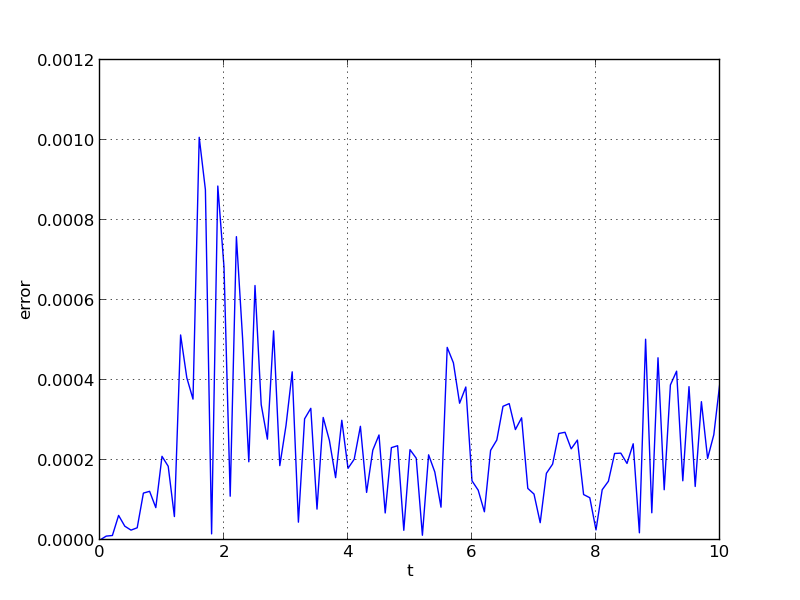
\includegraphics[width=0.450\linewidth]{plot-ark_analytic_nonlin_error.png}


\section{ark\_brusselator}
\label{c_serial:ark-brusselator}\label{c_serial:id5}
We now wish to exercise the ARKode solvers on more challenging
nonlinear ODE systems.  The following test simulates a brusselator
problem from chemical kinetics, and is widely used as a standard
benchmark problem for new solvers.  The ODE system has 3 components,
\(Y = [u,\, v,\, w]\), satisfying the equations,
\begin{gather}
\begin{split}\frac{du}{dt} &= a - (w+1)u + v u^2, \\
\frac{dv}{dt} &= w u - v u^2, \\
\frac{dw}{dt} &= \frac{b-w}{\varepsilon} - w u.\end{split}\notag
\end{gather}
We integrate over the interval \(0 \le t \le 10\), with the
initial conditions \(u(0) = u_0\), \(v(0) = v_0\), \(w(0)
= w_0\). After each unit time interval, the solution is output to the
screen.

The problem implements 3 different testing scenarios:

Test 1:  \(u_0=3.9\),  \(v_0=1.1\),  \(w_0=2.8\),
\(a=1.2\), \(b=2.5\), and \(\varepsilon=10^{-5}\)

Test 2:  \(u_0=1.2\), \(v_0=3.1\), \(w_0=3\), \(a=1\),
\(b=3.5\), and \(\varepsilon=5\cdot10^{-6}\)

Test 3:  \(u_0=3\), \(v_0=3\), \(w_0=3.5\), \(a=0.5\),
\(b=3\), and \(\varepsilon=5\cdot10^{-4}\)

The example problem currently selects test 2, though that value may be
easily adjusted to explore different testing scenarios.


\subsection{Numerical method}
\label{c_serial:id6}
This program solves the problem with the DIRK method, using a
Newton iteration with the SUNLINSOL\_DENSE linear solver module via
the ARKDLS interface.  Additionally, this example provides a routine
to ARKDLS to compute the dense Jacobian.

The problem is run using scalar relative and absolute tolerances of
\(rtol=10^{-6}\) and \(atol=10^{-10}\), respectively.

10 outputs are printed at equal intervals, and run statistics
are printed at the end.


\subsection{Solutions}
\label{c_serial:id7}
The computed solutions will of course depend on which test is
performed:

Test 1:  Here, all three components exhibit a rapid transient change
during the first 0.2 time units, followed by a slow and smooth
evolution.

Test 2: Here, \(w\) experiences a fast initial transient, jumping
0.5 within a few steps.  All values proceed smoothly until around
\(t=6.5\), when both \(u\) and \(v\) undergo a sharp
transition, with \(u\) increaseing from around 0.5 to 5 and
\(v\) decreasing from around 6 to 1 in less than 0.5 time units.
After this transition, both \(u\) and \(v\) continue to evolve
somewhat rapidly for another 1.4 time units, and finish off smoothly.

Test 3: Here, all components undergo very rapid initial transients
during the first 0.3 time units, and all then proceed very smoothly
for the remainder of the simulation.

Unfortunately, there are no known analytical solutions to the
Brusselator problem, but the following results have been verified
in code comparisons against both CVODE and the built-in ODE solver
\code{ode15s} from Matlab:

\includegraphics[width=0.300\linewidth]{plot-ark_brusselator1.png}

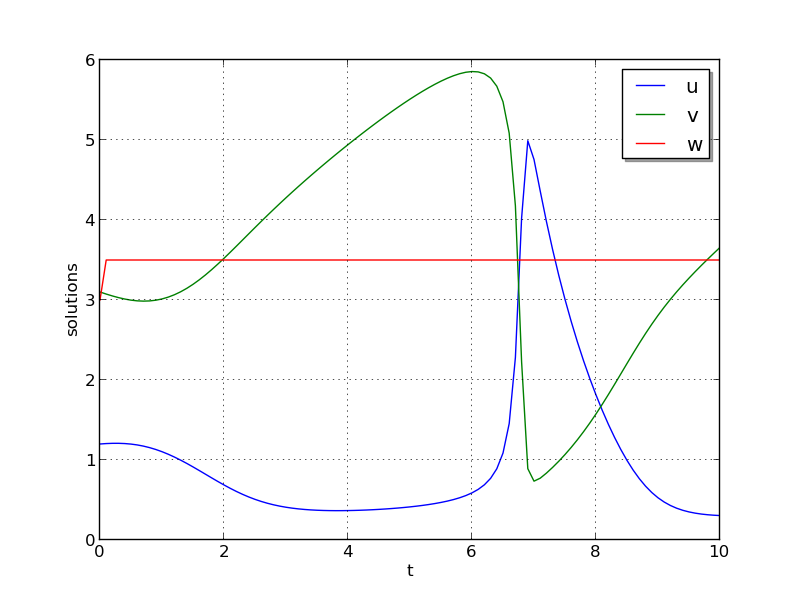
\includegraphics[width=0.300\linewidth]{plot-ark_brusselator2.png}

\includegraphics[width=0.300\linewidth]{plot-ark_brusselator3.png}

Brusselator solution plots: left is test 1, center is test 2, right is
test 3.


\section{ark\_brusselator\_fp}
\label{c_serial:ark-brusselator-fp}\label{c_serial:id8}
This test problem is a duplicate of the \code{ark\_brusselator} problem
above, but with a few key changes in the methods used for time
integration and nonlinear solver.  As with the previous test, this
problem has 3 dependent variables \(u\), \(v\) and \(w\),
that depend on the independent variable \(t\) via the IVP system
\begin{gather}
\begin{split}\frac{du}{dt} &= a - (w+1)u + v u^2, \\
\frac{dv}{dt} &= w u - v u^2, \\
\frac{dw}{dt} &= \frac{b-w}{\varepsilon} - w u.\end{split}\notag
\end{gather}
We integrate over the interval \(0 \le t \le 10\), with the
initial conditions \(u(0) = u_0\), \(v(0) = v_0\),
\(w(0) = w_0\).  After each unit time interval, the solution is
output to the screen.

Again, we have 3 different testing scenarios,

Test 1:  \(u_0=3.9\),  \(v_0=1.1\),  \(w_0=2.8\),
\(a=1.2\), \(b=2.5\), and \(\varepsilon=10^{-5}\)

Test 2:  \(u_0=1.2\), \(v_0=3.1\), \(w_0=3\), \(a=1\),
\(b=3.5\), and \(\varepsilon=5\cdot10^{-6}\)

Test 3:  \(u_0=3\), \(v_0=3\), \(w_0=3.5\), \(a=0.5\),
\(b=3\), and \(\varepsilon=5\cdot10^{-4}\)

with test 2 selected within in the example file.


\subsection{Numerical method}
\label{c_serial:id9}
This program solves the problem with the ARK method, in which we have
split the right-hand side into stiff (\(f_i(t,y)\)) and non-stiff
(\(f_e(t,y)\)) components,
\begin{gather}
\begin{split}f_i(t,y) = \left[\begin{array}{c}
   0 \\ 0 \\ \frac{b-w}{\varepsilon}
\end{array}\right]
\qquad
f_e(t,y) = \left[\begin{array}{c}
   a - (w+1)u + v u^2 \\ w u - v u^2 \\ - w u
\end{array}\right].\end{split}\notag
\end{gather}
Also unlike the previous test problem, we solve the resulting implicit
stages using the available accelerated fixed-point solver, enabled
through a call to \code{ARKodeSetFixedPoint}, with an acceleration
subspace of dimension 3.

10 outputs are printed at equal intervals, and run statistics
are printed at the end.


\section{ark\_brusselator\_mri}
\label{c_serial:id10}\label{c_serial:ark-brusselator-mri}
This test problem is a duplicate of the \code{ark\_brusselator} problem
above, but using MRIStep with different parameters.  As with the
previous test, this problem has 3 dependent variables \(u\), \(v\) and
\(w\), that depend on the independent variable \(t\) via the IVP system
\begin{gather}
\begin{split}\frac{du}{dt} &= a - (w+1)u + v u^2, \\
\frac{dv}{dt} &= w u - v u^2, \\
\frac{dw}{dt} &= \frac{b-w}{\varepsilon} - w u.\end{split}\notag
\end{gather}
We integrate over the interval \(0 \le t \le 2\), with the
initial conditions \(u(0) = u_0\), \(v(0) = v_0\), \(w(0)
= w_0\).  The solution is output to the screen at equal intervals of 0.1 time
units.

The problem implements the following testing scenario: \(u_0=1.2\),
\(v_0=3.1\),  \(w_0=3\), \(a=1\), \(b=3.5\), and
\(\varepsilon=10^{-2}\)


\subsection{Numerical method}
\label{c_serial:id11}
This program solves the problem with the default thrid order method.

The problem is run using a fixed slow step size \(hs=0.025\) and fast step
size \(0.001\).

20 outputs are printed at equal intervals, and run statistics
are printed at the end.


\section{ark\_robertson}
\label{c_serial:ark-robertson}\label{c_serial:id12}
Our next two tests simulate the Robertson problem, corresponding to the
kinetics of an autocatalytic reaction, corresponding to the CVODE
example of the same name.  This is an ODE system with 3
components, \(Y = [u,\, v,\, w]^T\), satisfying the equations,
\begin{gather}
\begin{split}\frac{du}{dt} &= -0.04 u + 10^4 v w, \\
\frac{dv}{dt} &= 0.04 u - 10^4 v w - 3\cdot10^7 v^2, \\
\frac{dw}{dt} &= 3\cdot10^7 v^2.\end{split}\notag
\end{gather}
We integrate over the interval \(0\le t\le 10^{11}\), with initial
conditions  \(Y(0) = [1,\, 0,\, 0]^T\).


\subsection{Numerical method}
\label{c_serial:id13}
This program is constructed to solve the problem with the DIRK solver.
Implicit subsystems are solved using a Newton iteration with the
SUNLINSOL\_DENSE dense linear solver module via the ARKDLS interface; a
routine is provided to ARKDLS to supply the Jacobian matrix.

The problem is run using scalar relative and absolute tolerances of
\(rtol=10^{-4}\) and \(atol=10^{-11}\), respectively.

100 outputs are printed at equal intervals, and run statistics are
printed at the end.


\subsection{Solutions}
\label{c_serial:id14}
Due to the linearly-spaced requested output times in this example, and
since we plot in a log-log scale, by the first output at
\(t=10^9\), the solutions have already undergone a sharp
transition from their initial values of \((u,v,w) = (1, 0, 0)\).
For additional detail on the early evolution of this problem, see the
following example, that requests logarithmically-spaced output times.

From the plot here, it is somewhat difficult to see the solution
values for \(w\), which here all have a value of
\(1 \pm 10^{-5}\).  Additionally, we see that near the end of the
evolution, the values for \(v\) begin to exhibit oscillations;
this is due to the fact that by this point those values have fallen
below their specified absolute tolerance.  A smoother behavior (with
an increase in time steps) may be obtained by reducing the absolute
tolerance for that variable.
\begin{figure}[htbp]
\centering

\scalebox{0.700000}{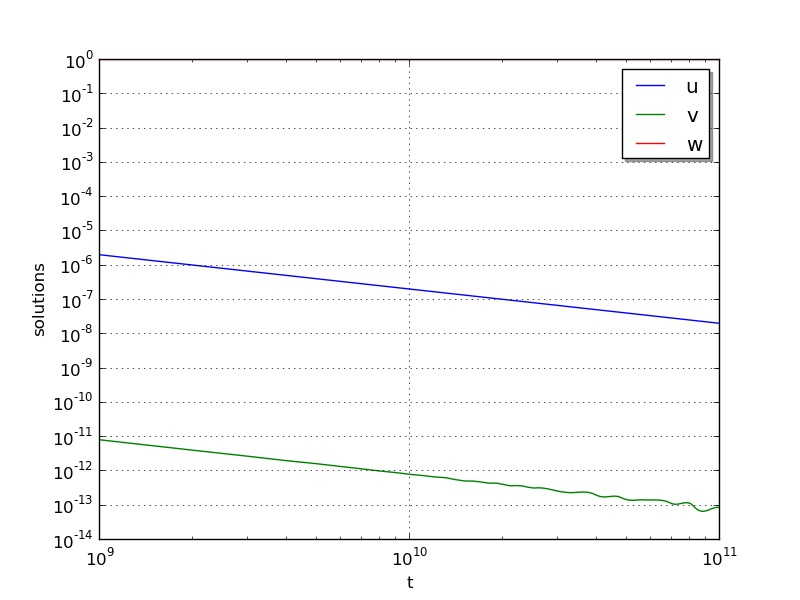
\includegraphics{plot-ark_robertson.png}}
\end{figure}


\section{ark\_robertson\_root}
\label{c_serial:ark-robertson-root}\label{c_serial:id15}
We again test the Robertson problem, but in this example we will
utilize both a logarithmically-spaced set of output times (to properly
show the solution behavior), as well as ARKode's root-finding
capabilities.  Again, the Robertson problem consists of an ODE system
with 3 components, \(Y = [u,\, v,\, w]^T\), satisfying the equations,
\begin{gather}
\begin{split}\frac{du}{dt} &= -0.04 u + 10^4 v w, \\
\frac{dv}{dt} &= 0.04 u - 10^4 v w - 3\cdot10^7 v^2, \\
\frac{dw}{dt} &= 3\cdot10^7 v^2.\end{split}\notag
\end{gather}
We integrate over the interval \(0\le t\le 10^{11}\), with initial
conditions  \(Y(0) = [1,\, 0,\, 0]^T\).

Additionally, we supply the following two root-finding equations:
\begin{gather}
\begin{split}g_1(u) = u - 10^{-4}, \\
g_2(w) = w - 10^{-2}.\end{split}\notag
\end{gather}
While these are not inherently difficult nonlinear equations, they
easily serve the purpose of determining the times at which our
solutions attain desired target values.


\subsection{Numerical method}
\label{c_serial:id16}
This program solves the problem with the DIRK solver.  Implicit
subsystems are solved using a Newton iteration with the
SUNLINSOL\_DENSE linear solver module via the ARKDLS interface; a
routine is supplied to provide the dense Jacobian matrix.

The problem is run using scalar relative and vector absolute
tolerances.  Here, we choose relative tolerance \(rtol=10^{-4}\),
and set absolute tolerances on \(u\), \(v\) and \(w\) of
\(10^{-8}\), \(10^{-11}\) and \(10^{-8}\), respectively.

100 outputs are printed at equal intervals, and run statistics are
printed at the end.

However, unlike in the previous problem, while integrating the system,
we use the rootfinding feature of ARKode to find the times at which
either \(u=10^{-4}\) or \(w=10^{-2}\).


\subsection{Solutions}
\label{c_serial:id17}
In the solutions below, we now see the early-time evolution of the
solution components for the Robertson ODE system.
\begin{figure}[htbp]
\centering

\scalebox{0.700000}{\includegraphics{plot-ark_robertson_root.png}}
\end{figure}

We note that when running this example, the root-finding capabilities
of ARKode report outside of the typical logarithmically-spaced output
times to declare that at time \(t=0.264019\) the variable
\(w\) attains the value \(10^{-2}\), and that at time
\(t=2.07951\cdot10^{7}\) the variable \(u\) attains the value
\(10^{-4}\); both of our thresholds specified by the root-finding
function \code{g()}.


\section{ark\_brusselator1D}
\label{c_serial:id18}\label{c_serial:ark-brusselator1d}
We now investigate a time-dependent system of partial differential
equations.  We adapt the previously-described brusselator test problem
by adding diffusion into the chemical reaction network.  We again have
a system with 3 components, \(Y = [u,\, v,\, w]^T\) that satisfy
the equations,
\begin{gather}
\begin{split}\frac{\partial u}{\partial t} &= d_u \frac{\partial^2 u}{\partial
   x^2} + a - (w+1) u + v u^2, \\
\frac{\partial v}{\partial t} &= d_v \frac{\partial^2 v}{\partial
   x^2} + w u - v u^2, \\
\frac{\partial w}{\partial t} &= d_w \frac{\partial^2 w}{\partial
   x^2} + \frac{b-w}{\varepsilon} - w u.\end{split}\notag
\end{gather}
However, now these solutions are also spatially dependent.  We
integrate for \(t \in [0, 10]\), and \(x \in [0, 1]\), with
initial conditions
\begin{gather}
\begin{split}u(0,x) &=  a + \frac{1}{10} \sin(\pi x),\\
v(0,x) &= \frac{b}{a} + \frac{1}{10}\sin(\pi x),\\
w(0,x) &=  b + \frac{1}{10}\sin(\pi x),\end{split}\notag
\end{gather}
and with stationary boundary conditions, i.e.
\begin{gather}
\begin{split}\frac{\partial u}{\partial t}(t,0) &= \frac{\partial u}{\partial t}(t,1) = 0,\\
\frac{\partial v}{\partial t}(t,0) &= \frac{\partial v}{\partial t}(t,1) = 0,\\
\frac{\partial w}{\partial t}(t,0) &= \frac{\partial w}{\partial t}(t,1) = 0.\end{split}\notag
\end{gather}
We note that these can also be implemented as Dirichlet boundary
conditions with values identical to the initial conditions.


\subsection{Numerical method}
\label{c_serial:id19}
We employ a \emph{method of lines} approach, wherein we first
semi-discretize in space to convert the system of 3 PDEs into a larger
system of ODEs.  To this end, the spatial derivatives are computed
using second-order centered differences, with the data distributed
over \(N\) points on a uniform spatial grid.  As a result, ARKode
approaches the problem as one involving \(3N\) coupled ODEs.

The problem is run using \(N=201\) spatial points, with parameters
\(a=0.6\), \(b=2.0\), \(d_u=0.025\), \(d_v=0.025\),
\(d_w=0.025\) and \(\varepsilon=10^{-5}\).  We specify scalar
relative and absolute solver tolerances of \(rtol=10^{-6}\) and
\(atol=10^{-10}\), respectively.

This program solves the problem with a DIRK method, using a Newton
iteration with the SUNLINSOL\_BAND linear solver module via the ARKDLS
interface; a routine is supplied to fill the banded Jacobian matrix.

100 outputs are printed at equal intervals, and run statistics
are printed at the end.


\subsection{Solutions}
\label{c_serial:id20}
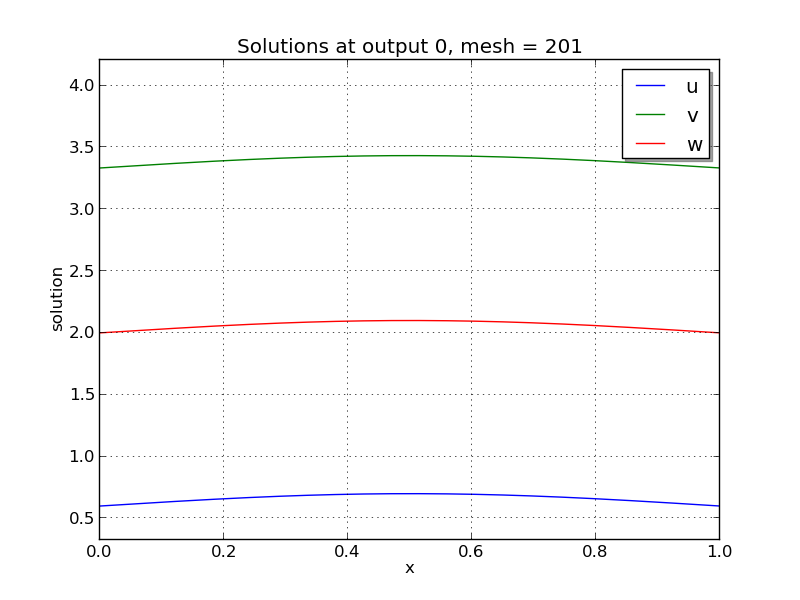
\includegraphics[width=0.300\linewidth]{plot-ark_brusselator1D_1.png}

\includegraphics[width=0.300\linewidth]{plot-ark_brusselator1D_2.png}

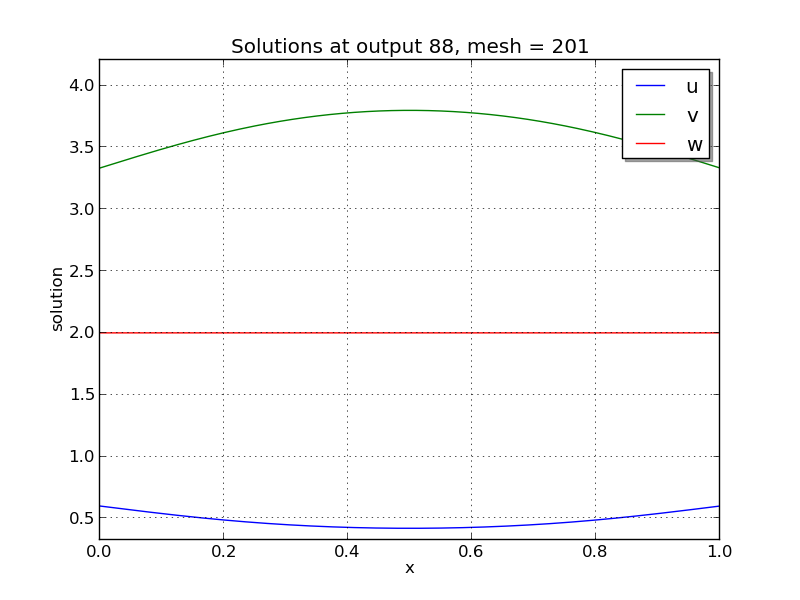
\includegraphics[width=0.300\linewidth]{plot-ark_brusselator1D_3.png}

Brusselator PDE solution snapshots: left is at time \(t=0\),
center is at time \(t=2.9\), right is at time \(t=8.8\).


\section{ark\_brusselator1D\_klu}
\label{c_serial:ark-brusselator1d-klu}\label{c_serial:id21}
This problem is mathematically identical to the preceding problem,
{\hyperref[c_serial:ark-brusselator1d]{\emph{\DUspan{}{ark\_brusselator1D}}}}, but instead of using the SUNMATRIX\_BAND
banded matrix module and SUNLINSOL\_BAND linear solver module, it uses
the SUNMATRIX\_SPARSE sparse matrix module with the SUNLINSOL\_KLU
linear solver module.  These are still provided to ARKode using the
ARKDLS direct linear solver interface, and again a routine is provided
to supply a compressed-sparse-column version of the Jacobian matrix.
Additionally, the solution is only output 10 times instead of 100.


\section{ark\_brusselator1D\_FEM\_slu}
\label{c_serial:ark-brusselator1d-fem-slu}\label{c_serial:id22}
This problem is mathematically identical to the preceding problems,
{\hyperref[c_serial:ark-brusselator1d]{\emph{\DUspan{}{ark\_brusselator1D}}}} and {\hyperref[c_serial:ark-brusselator1d-klu]{\emph{\DUspan{}{ark\_brusselator1D\_klu}}}}, but
utilizes a different set of numerical methods.


\subsection{Numerical method}
\label{c_serial:id23}
As with the preceding problems, we employ a method of lines approach,
wherein we first semi-discretize in space to convert the system of 3
PDEs into a larger system of ODEs.  However, in this example we
discretize in space using a standard piecewise linear, Galerkin finite
element method, over a non-uniform discretization of the interval
\([0,1]\) into 100 subintervals.  To this end, we must integrate
each term in each equation, multiplied by test functions, over each
subinterval, e.g.
\begin{gather}
\begin{split}\int_{x_i}^{x_{i+1}} \left(a - (w+1) u + v u^2\right) \varphi\,\mathrm dx.\end{split}\notag
\end{gather}
Since we employ piecewise linear basis and trial functions, the
highest nonlinearity in the model is a quartic polynomial.  We
therefore approximate these integrals using a three-node Gaussian
quadrature, exact for polynomials up to degree six.

After this spatial semi-discretization, the system of three PDEs is
passed to ARKode as a system of \(3N\) coupled ODEs, as with the
preceding problem.

As with the preceding problem {\hyperref[c_serial:ark-brusselator1d-klu]{\emph{\DUspan{}{ark\_brusselator1D\_klu}}}}, this
example solves the problem with a DIRK method, using a Newton
iteration, and the SUNMATRIX\_SPARSE module.  However, this example
uses the SUNLINSOL\_SUPERLUMT linear solver module, both for the Newton
systems having Jacobian \(A=M-\gamma J\), as well as for the
mass-matrix-only linear systems with matrix \(M\).  Functions
implementing both \(J\) and \(M\) in compressed-sparse-column
format are supplied.

100 outputs are printed at equal intervals, and run statistics
are printed at the end.


\subsection{Solutions}
\label{c_serial:id24}
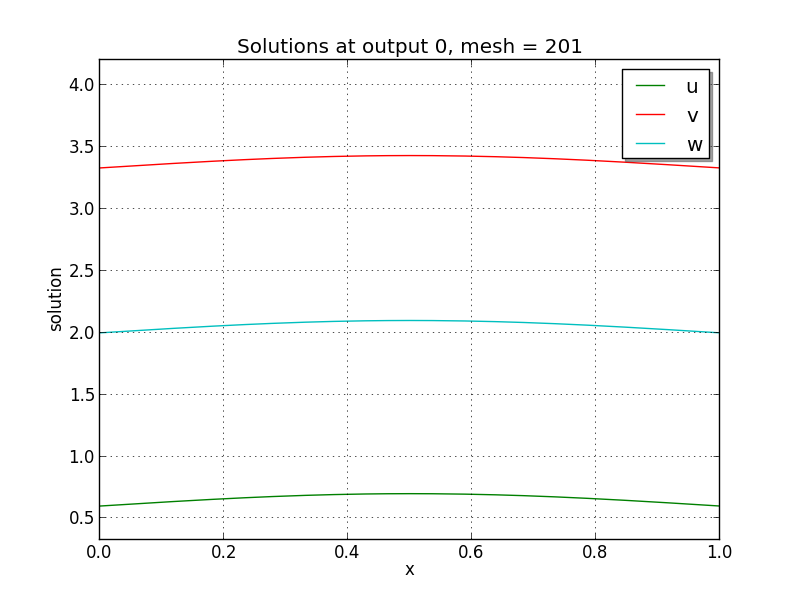
\includegraphics[width=0.300\linewidth]{plot-ark_brusselator1D_FEM_1.png}

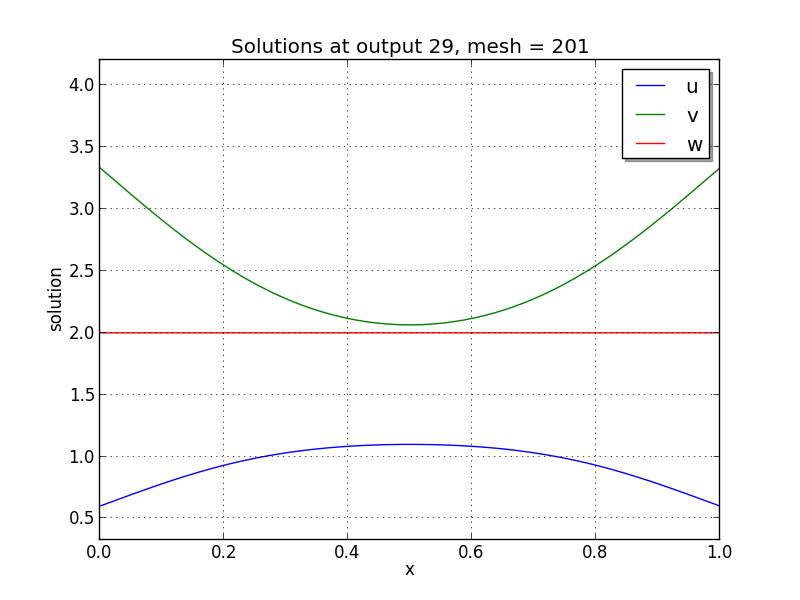
\includegraphics[width=0.300\linewidth]{plot-ark_brusselator1D_FEM_2.png}

\includegraphics[width=0.300\linewidth]{plot-ark_brusselator1D_FEM_3.png}

Finite-element Brusselator PDE solution snapshots (created using the
supplied Python script, \code{plot\_brusselator1D\_FEM.py}): left is at time
\(t=0\), center is at time \(t=2.9\), right is at time
\(t=8.8\).


\section{ark\_heat1D}
\label{c_serial:ark-heat1d}\label{c_serial:id25}
As with the previous brusselator problem, this example simulates a
simple one-dimensional partial differential equation; in this case we
consider the heat equation,
\begin{gather}
\begin{split}\frac{\partial u}{\partial t} = k \frac{\partial^2 u}{\partial x^2} + f,\end{split}\notag
\end{gather}
for \(t \in [0, 10]\), and \(x \in [0, 1]\), with initial
condition \(u(0,x) = 0\), stationary boundary conditions,
\begin{gather}
\begin{split}\frac{\partial u}{\partial t}(t,0) = \frac{\partial u}{\partial t}(t,1) = 0,\end{split}\notag
\end{gather}
and a point-source heating term,
\begin{gather}
\begin{split}f(t,x) = \begin{cases} 1 & \text{if}\;\; x=1/2, \\
                       0 & \text{otherwise}. \end{cases}\end{split}\notag
\end{gather}

\subsection{Numerical method}
\label{c_serial:id26}
As with the {\hyperref[c_serial:ark-brusselator1d]{\emph{\DUspan{}{ark\_brusselator1D}}}} test problem, this test computes
spatial derivatives using second-order centered differences, with the
data distributed over \(N\) points on a uniform spatial grid.

In this example, we use \(N=201\) spatial points, with heat
conductivity parameter \(k=0.5\), and discretize the equation
using second-order centered finite-differences.  The problem is run
using scalar relative and absolute solver tolerances of
\(rtol=10^{-6}\) and \(atol=10^{-10}\), respectively.

This program solves the problem with a DIRK method, utilizing a Newton
iteration.  The primary utility in including this example is that
since the Newton linear systems are now symmetric, we solve these
using the SUNLINSOL\_PCG iterative linear solver, through the ARKSPILS
linear solver interface.  A routine to perform the Jacobian-vector
product routine is supplied, in order to provide an example of its use.


\subsection{Solutions}
\label{c_serial:id27}
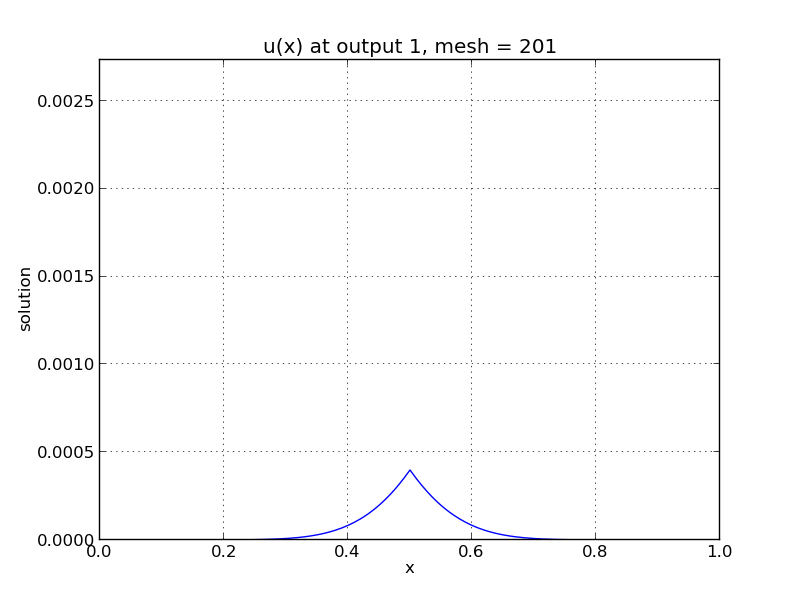
\includegraphics[width=0.300\linewidth]{plot-ark_heat1d_1.png}

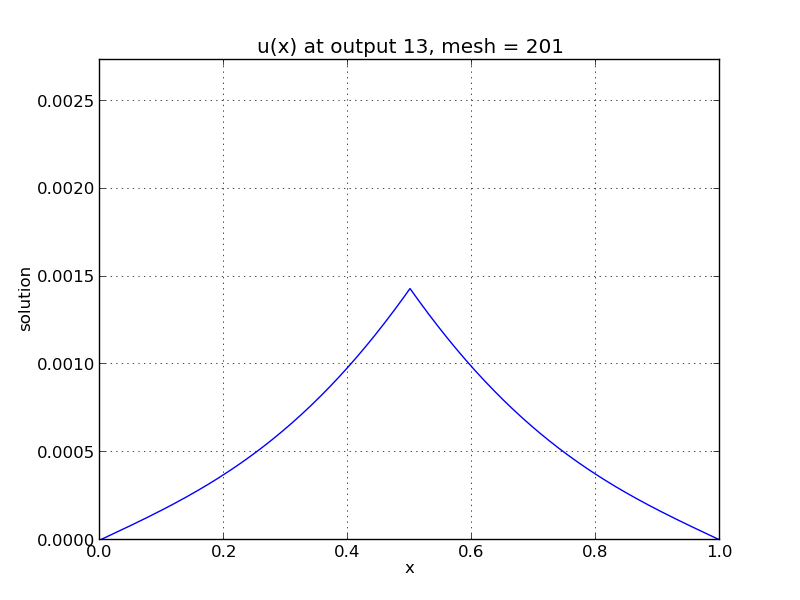
\includegraphics[width=0.300\linewidth]{plot-ark_heat1d_2.png}

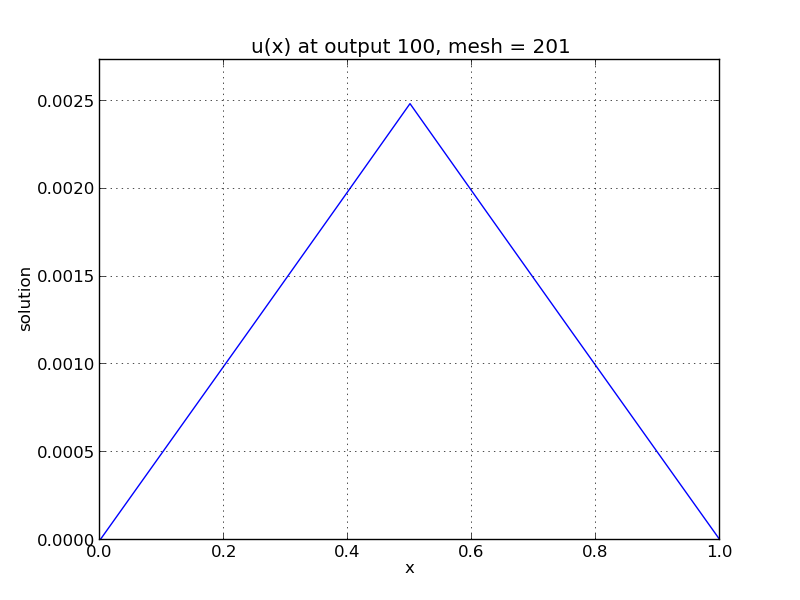
\includegraphics[width=0.300\linewidth]{plot-ark_heat1d_3.png}

One-dimensional heat PDE solution snapshots: left is at time \(t=0.01\),
center is at time \(t=0.13\), right is at time \(t=1.0\).


\section{ark\_heat1D\_adapt}
\label{c_serial:id28}\label{c_serial:ark-heat1d-adapt}
This problem is mathematically identical to the {\hyperref[c_serial:ark-heat1d]{\emph{\DUspan{}{ark\_heat1D}}}} test
problem.  However, instead of using a uniform spatial grid, this test
problem utilizes a dynamically-evolving spatial mesh.  The PDE under
consideration is a simple one-dimensional heat equation,
\begin{gather}
\begin{split}\frac{\partial u}{\partial t} = k \frac{\partial^2 u}{\partial x^2} + f,\end{split}\notag
\end{gather}
for \(t \in [0, 10]\), and \(x \in [0, 1]\), with initial
condition \(u(0,x) = 0\), stationary boundary conditions,
\begin{gather}
\begin{split}\frac{\partial u}{\partial t}(t,0) = \frac{\partial u}{\partial t}(t,1) = 0,\end{split}\notag
\end{gather}
and a point-source heating term,
\begin{gather}
\begin{split}f(t,x) = \begin{cases} 1 & \text{if}\;\; x=1/2, \\
                       0 & \text{otherwise}. \end{cases}\end{split}\notag
\end{gather}

\subsection{Numerical method}
\label{c_serial:id29}
We again employ a method-of-lines discretization approach.  The
spatial derivatives are computed using a three-point centered stencil,
that is accurate to \(O(\Delta x_i^2)\) if the neighboring points are
equidistant from the central point, i.e. \(x_{i+1} - x_i = x_i -
x_{i-1}\); however, if these neighbor distances are unequal the
approximation reduces to first-order accuracy.  The spatial mesh is
initially distributed uniformly over 21 points in \([0,1]\), but
as the simulation proceeds the mesh is {[}crudely{]} adapted to add points
to the center of subintervals bordering any node where
\(\left|\frac{\partial^2 u}{\partial x^2}\right| > 0.003\).
We note that the spatial adaptivity approach employed in this example
is \emph{ad-hoc}, designed only to exemplify ARKode usage on a problem with
varying size (not to show optimally-adaptive spatial refinement
methods).

This program solves the problem with a DIRK method, utilizing a Newton
iteration and the SUNLINSOL\_PCG iterative linear solver.
Additionally, the test problem utilizes ARKode's spatial adaptivity
support (via \code{ARKodeResize}), allowing retention of the
major ARKode data structures across vector length changes.


\section{ark\_KrylovDemo\_prec}
\label{c_serial:ark-krylovdemo-prec}\label{c_serial:id30}
This problem is an ARKode clone of the CVODE problem,
\code{cv\_KrylovDemo\_prec}.  This is a demonstration program using the
SUNLINSOL\_SPGMR linear solver module.  As explained more thoroughly in
\phantomsection\label{c_serial:id31}{\hyperref[References:hsr2017]{\emph{{[}HSR2017{]}}}}, the problem is a stiff ODE system that arises from a
system of PDEs modeling a six-species food web population model, with
predator-prey interaction and diffusion on the unit square in two
dimensions.  We have a system with 6 components, \(C = [c^1,\,
c^2,\,\ldots, c^6]^T\) that satisfy the equations,
\begin{gather}
\begin{split}\frac{\partial c^i}{\partial t} &= d_i \left(\frac{\partial^2 c^i}{\partial
   x^2} + \frac{\partial^2 c^i}{\partial y^2}\right) +
   f_i(x,y,c),\quad i=1,\ldots,6.\end{split}\notag
\end{gather}
where
\begin{gather}
\begin{split}f_i(x,y,c) = c^i\left( b_i + \sum_{j=1}^{ns} a_{i,j} c^j\right).\end{split}\notag
\end{gather}
Here, the first three species are prey and the last three are
predators.  The coefficients \(a_{i,j}, b_i, d_i\) are:
\begin{gather}
\begin{split}a_{i,j} = \begin{cases}
            -1, \quad & i=j,\\
            -0.5\times10^{-6}, \quad & i\le 3, j>3, \\
             10^4, \quad & i>3, j\le3
          \end{cases}
b_i = \begin{cases}
         (1+xy), \quad & i\le 3,\\
        -(1+xy), \quad & i>3
      \end{cases}
d_i = \begin{cases}
         1, \quad & i\le 3,\\
         \frac12, \quad & i>3
      \end{cases}\end{split}\notag
\end{gather}
The spatial domain is \((x,y) \in [0, 1]^2\); the time domain is
\(t \in [0,10]\), with initial conditions
\begin{gather}
\begin{split}c^i(x,y) &=  10 + i \sqrt{4x(1-x)}\sqrt{4y(1-y)}\end{split}\notag
\end{gather}
and with homogeneous Neumann boundary conditions,
\(\nabla c^i \cdot \vec{n} = 0\).


\subsection{Numerical method}
\label{c_serial:id32}
We employ a method of lines approach, wherein we first semi-discretize
in space to convert the system of 6 PDEs into a larger system of ODEs.
To this end, the spatial derivatives are computed using second-order
centered differences, with the data distributed over \(Mx*My\)
points on a uniform spatial grid.  As a result, ARKode approaches the
problem as one involving \(6*Mx*My\) coupled ODEs.

This program solves the problem with a DIRK method, using a Newton
iteration with the preconditioned SUNLINSOL\_SPGMR iterative linear
solver module, and ARKSPILS interface.  The preconditioner matrix used
is the product of two matrices:
\begin{enumerate}
\item {} 
A matrix, only defined implicitly, based on a fixed number of
Gauss-Seidel iterations using the diffusion terms only.

\item {} 
A block-diagonal matrix based on the partial derivatives of the
interaction terms \(f\) only, using block-grouping (computing
only a subset of the \(3\times3\) blocks).

\end{enumerate}

Four different runs are made for this problem.  The product
preconditoner is applied on the left and on the right.  In each case,
both the modified and classical Gram-Schmidt orthogonalization options
are tested.  In the series of runs, \code{ARKodeInit}, \code{SUNSPGMR},
\code{ARKSpilsSetLinearSolver}, \code{SUNSPGMRSetGSType},
\code{ARKSpilsSetEpsLin} and \code{ARKSpilsSetPreconditioner} are called
only for the first run, whereas \code{ARKodeReInit},
\code{SUNSPGMRSetPrecType} and \code{SUNSPGMRSetGSType} are called to
re-initialize the integrator and update linear solver parameters for
each of the remaining three runs.

A problem description, performance statistics at selected output
times, and final statistics are written to standard output.  On the
first run, solution values are also printed at output times.  Error
and warning messages are written to standard error, but there should
be no such messages.


\section{ark\_onewaycouple\_mri}
\label{c_serial:ark-onewaycouple-mri}\label{c_serial:id33}
This example simulates a linear system of 3 dependent variables \(u\),
\(v\) and \(w\), that depend on the independent variable \(t\) via
the IVP system
\begin{gather}
\begin{split}\frac{du}{dt} &= -50 v, \\
\frac{dv}{dt} &= 50 u, \\
\frac{dw}{dt} &= -w + u + v.\end{split}\notag
\end{gather}
We integrate over the interval \(0 \le t \le 1\), with the initial
conditions \(u(0) = 1\), \(v(0) = 0\), \(w(0)= 2\).  The
solution is output to the screen at equal intervals of 0.1 time units.


\subsection{Numerical method}
\label{c_serial:id34}
This program solves the problem with the default third order method.

The problem is run using a fixed slow step size \(hs=0.001\) and fast step
size \(0.0001\).

10 outputs are printed at equal intervals, and run statistics
are printed at the end.


\subsection{Solutions}
\label{c_serial:id35}
This system has the analytic solution,
\begin{gather}
\begin{split}u(t) &= \cos(50t), \\
v(t) &= \sin(50t), \\
w(t) &= 5051/2501*\exp(-t) - 49/2501*\cos(50t) + 51/2501*\sin(50t).\end{split}\notag
\end{gather}

\section{ark\_twowaycouple\_mri}
\label{c_serial:id36}\label{c_serial:ark-twowaycouple-mri}
This example simulates a linear system of 3 dependent variables \(u\),
\(v\) and \(w\), that depend on the independent variable \(t\) via
the IVP system
\begin{gather}
\begin{split}\frac{du}{dt} &= 100 v + w, \\
\frac{dv}{dt} &= -100 u, \\
\frac{dw}{dt} &= -w + u.\end{split}\notag
\end{gather}
We integrate over the interval \(0 \le t \le 2\), with the initial
conditions \(u(0) = 9001/10001\), \(v(0) = 10^{-5}/10001\),
\(w(0)= 1000\).  The solution is output to the screen at equal intervals of
0.1 time units.


\subsection{Numerical method}
\label{c_serial:id37}
This program solves the problem with the default third order method.

The problem is run using a fixed slow step size \(hs=0.001\) and fast step
size \(0.00002\).

20 outputs are printed at equal intervals, and run statistics
are printed at the end.


\chapter{OpenMP C example problems}
\label{c_openmp:openmp-c}\label{c_openmp::doc}\label{c_openmp:openmp-c-example-problems}

\section{ark\_brusselator1D\_omp}
\label{c_openmp:ark-brusselator1d-omp}\label{c_openmp:id1}
This problem is mathematically identical to the one-dimensional
reaction-diffusion brusselator model, {\hyperref[c_serial:ark-brusselator1d]{\emph{\DUspan{}{ark\_brusselator1D}}}}.  As
before, we investigate a time-dependent system of partial differential
equations with 3 components, \(Y = [u,\, v,\, w]^T\) that satisfy
the equations,
\begin{gather}
\begin{split}\frac{\partial u}{\partial t} &= d_u \frac{\partial^2 u}{\partial
   x^2} + a - (w+1) u + v u^2, \\
\frac{\partial v}{\partial t} &= d_v \frac{\partial^2 v}{\partial
   x^2} + w u - v u^2, \\
\frac{\partial w}{\partial t} &= d_w \frac{\partial^2 w}{\partial
   x^2} + \frac{b-w}{\varepsilon} - w u.\end{split}\notag
\end{gather}
We integrate for \(t \in [0, 10]\), and \(x \in [0, 1]\), with
initial conditions
\begin{gather}
\begin{split}u(0,x) &=  a + \frac{1}{10} \sin(\pi x),\\
v(0,x) &= \frac{b}{a} + \frac{1}{10}\sin(\pi x),\\
w(0,x) &=  b + \frac{1}{10}\sin(\pi x),\end{split}\notag
\end{gather}
and with stationary boundary conditions, i.e.
\begin{gather}
\begin{split}\frac{\partial u}{\partial t}(t,0) &= \frac{\partial u}{\partial t}(t,1) = 0,\\
\frac{\partial v}{\partial t}(t,0) &= \frac{\partial v}{\partial t}(t,1) = 0,\\
\frac{\partial w}{\partial t}(t,0) &= \frac{\partial w}{\partial t}(t,1) = 0.\end{split}\notag
\end{gather}

\subsection{Numerical method}
\label{c_openmp:numerical-method}
The numerical method is identical to the previous implementation,
except that we now use SUNDIALS' OpenMP-enabled vector kernel module,
NVECTOR\_OPENMP, and have similarly threaded the supplied right-hand
side and banded Jacobian construction functions.


\chapter{Parallel C example problems}
\label{c_parallel::doc}\label{c_parallel:parallel-c-example-problems}\label{c_parallel:parallel-c}

\section{ark\_diurnal\_kry\_bbd\_p}
\label{c_parallel:ark-diurnal-kry-bbd-p}\label{c_parallel:id1}
This problem is an ARKode clone of the CVODE problem,
\code{cv\_diurnal\_kry\_bbd\_p}.  As described in \phantomsection\label{c_parallel:id2}{\hyperref[References:hsr2017]{\emph{{[}HSR2017{]}}}}, this problem
models a two-species diurnal kinetics advection-diffusion PDE system
in two spatial dimensions,
\begin{gather}
\begin{split}\frac{\partial c_i}{\partial t} &=
  K_h \frac{\partial^2 c_i}{\partial x^2} +
  V \frac{\partial     c_i}{\partial x} +
  \frac{\partial}{\partial y}\left( K_v(y)
  \frac{\partial c_i}{\partial y}\right) +
  R_i(c_1,c_2,t),\quad i=1,2\end{split}\notag
\end{gather}
where
\begin{gather}
\begin{split}R_1(c_1,c_2,t) &= -q_1*c_1*c_3 - q_2*c_1*c_2 + 2*q_3(t)*c_3 + q_4(t)*c_2, \\
R_2(c_1,c_2,t) &=  q_1*c_1*c_3 - q_2*c_1*c_2 - q_4(t)*c_2, \\
K_v(y) &= K_{v0} e^{y/5}.\end{split}\notag
\end{gather}
Here \(K_h\), \(V\), \(K_{v0}\), \(q_1\), \(q_2\),
and \(c_3\) are constants, and \(q_3(t)\) and \(q_4(t)\)
vary diurnally.  The problem is posed on the square spatial domain
\((x,y) \in [0,20]\times[30,50]\), with homogeneous Neumann
boundary conditions, and for time interval \(t\in [0,86400]\) sec
(1 day).

We enforce the initial conditions
\begin{gather}
\begin{split}c_1(x,y) &=  10^6 \chi(x)\eta(y) \\
c_2(x,y) &=  10^{12} \chi(x)\eta(y) \\
\chi(x) &= 1 - \sqrt{\frac{x - 10}{10}} + \frac12 \sqrt[4]{\frac{x - 10}{10}} \\
\eta(y) &= 1 - \sqrt{\frac{y - 40}{10}} + \frac12 \sqrt[4]{\frac{x - 10}{10}}.\end{split}\notag
\end{gather}

\subsection{Numerical method}
\label{c_parallel:numerical-method}
We employ a method of lines approach, wherein we first
semi-discretize in space to convert the system of 2 PDEs into a larger
system of ODEs.  To this end, the spatial derivatives are computed
using second-order centered differences, with the data distributed
over \(Mx*My\) points on a uniform spatial grid.  As a result, ARKode
approaches the problem as one involving \(2*Mx*My\) coupled ODEs.

The problem is decomposed in parallel into uniformly-sized subdomains,
with two subdomains in each direction (four in total), and where each
subdomain has five points in each direction (i.e. \(Mx=My=10\)).

This program solves the problem with a DIRK method, using a Newton
iteration with the preconditioned SUNLINSOL\_SPGMR iterative linear
solver through the ARKSPILS interface.

The preconditioner matrix used is block-diagonal, with banded blocks,
constructed using the ARKBBDPRE module.  Each block is generated using
difference quotients, with half-bandwidths \code{mudq = mldq = 10}, but
the retained banded blocks have half-bandwidths \code{mukeep = mlkeep = 2}.
A copy of the approximate Jacobian is saved and conditionally reused
within the preconditioner routine.

Two runs are made for this problem, first with left and then with
right preconditioning.

Performance data and sampled solution values are printed at
selected output times, and all performance counters are printed
on completion.


\section{ark\_diurnal\_kry\_p}
\label{c_parallel:id3}\label{c_parallel:ark-diurnal-kry-p}
This problem is an ARKode clone of the CVODE problem,
\code{cv\_diurnal\_kry\_p}.  As described in \phantomsection\label{c_parallel:id4}{\hyperref[References:hsr2017]{\emph{{[}HSR2017{]}}}}, this test problem
models a two-species diurnal kinetics advection-diffusion PDE system
in two spatial dimensions,
\begin{gather}
\begin{split}\frac{\partial c_i}{\partial t} &=
  K_h \frac{\partial^2 c_i}{\partial x^2} +
  V \frac{\partial     c_i}{\partial x} +
  \frac{\partial}{\partial y}\left( K_v(y)
  \frac{\partial c_i}{\partial y}\right) +
  R_i(c_1,c_2,t),\quad i=1,2\end{split}\notag
\end{gather}
where
\begin{gather}
\begin{split}R_1(c_1,c_2,t) &= -q_1*c_1*c_3 - q_2*c_1*c_2 + 2*q_3(t)*c_3 + q_4(t)*c_2, \\
R_2(c_1,c_2,t) &=  q_1*c_1*c_3 - q_2*c_1*c_2 - q_4(t)*c_2, \\
K_v(y) &= K_{v0} e^{y/5}.\end{split}\notag
\end{gather}
Here \(K_h\), \(V\), \(K_{v0}\), \(q_1\), \(q_2\),
and \(c_3\) are constants, and \(q_3(t)\) and \(q_4(t)\)
vary diurnally.  The problem is posed on the square spatial domain
\((x,y) \in [0,20]\times[30,50]\), with homogeneous Neumann
boundary conditions, and for time interval \(t\in [0,86400]\) sec
(1 day).

We enforce the initial conditions
\begin{gather}
\begin{split}c^1(x,y) &=  10^6 \chi(x)\eta(y) \\
c^2(x,y) &=  10^{12} \chi(x)\eta(y) \\
\chi(x) &= 1 - \sqrt{\frac{x - 10}{10}} + \frac12 \sqrt[4]{\frac{x - 10}{10}} \\
\eta(y) &= 1 - \sqrt{\frac{y - 40}{10}} + \frac12 \sqrt[4]{\frac{x - 10}{10}}.\end{split}\notag
\end{gather}

\subsection{Numerical method}
\label{c_parallel:id5}
We employ a method of lines approach, wherein we first semi-discretize
in space to convert the system of 2 PDEs into a larger system of ODEs.
To this end, the spatial derivatives are computed using second-order
centered differences, with the data distributed over \(Mx*My\)
points on a uniform spatial grid.  As a result, ARKode approaches the
problem as one involving \(2*Mx*My\) coupled ODEs.

The problem is decomposed in parallel into uniformly-sized subdomains,
with two subdomains in each direction (four in total), and where each
subdomain has five points in each direction (i.e. \(Mx=My=10\)).

This program solves the problem with a DIRK method, using a Newton
iteration with the preconditioned SUNLINSOL\_SPGMR iterative linear
solver, through the ARKSPILS interface.

The preconditioner matrix used is block-diagonal, with block-diagonal
portion of the Newton matrix used as a left preconditioner.  A copy of
the block-diagonal portion of the Jacobian is saved and conditionally
reused within the preconditioner routine.

Performance data and sampled solution values are printed at
selected output times, and all performance counters are printed
on completion.


\chapter{Parallel Hypre example problems}
\label{c_parhyp:parhyp-c}\label{c_parhyp::doc}\label{c_parhyp:parallel-hypre-example-problems}

\section{ark\_diurnal\_kry\_ph}
\label{c_parhyp:ark-diurnal-kry-ph}\label{c_parhyp:id1}
This problem is mathematically identical to the parallel C example
problem {\hyperref[c_parallel:ark-diurnal-kry-p]{\emph{\DUspan{}{ark\_diurnal\_kry\_p}}}}.  As before, this test problem models
a two-species diurnal kinetics advection-diffusion PDE system in two
spatial dimensions,
\begin{gather}
\begin{split}\frac{\partial c_i}{\partial t} &=
  K_h \frac{\partial^2 c_i}{\partial x^2} +
  V \frac{\partial     c_i}{\partial x} +
  \frac{\partial}{\partial y}\left( K_v(y)
  \frac{\partial c_i}{\partial y}\right) +
  R_i(c_1,c_2,t),\quad i=1,2\end{split}\notag
\end{gather}
where
\begin{gather}
\begin{split}R_1(c_1,c_2,t) &= -q_1*c_1*c_3 - q_2*c_1*c_2 + 2*q_3(t)*c_3 + q_4(t)*c_2, \\
R_2(c_1,c_2,t) &=  q_1*c_1*c_3 - q_2*c_1*c_2 - q_4(t)*c_2, \\
K_v(y) &= K_{v0} e^{y/5}.\end{split}\notag
\end{gather}
Here \(K_h\), \(V\), \(K_{v0}\), \(q_1\), \(q_2\),
and \(c_3\) are constants, and \(q_3(t)\) and \(q_4(t)\)
vary diurnally.  The problem is posed on the square spatial domain
\((x,y) \in [0,20]\times[30,50]\), with homogeneous Neumann
boundary conditions, and for time interval \(t\in [0,86400]\) sec
(1 day).

We enforce the initial conditions
\begin{gather}
\begin{split}c^1(x,y) &=  10^6 \chi(x)\eta(y) \\
c^2(x,y) &=  10^{12} \chi(x)\eta(y) \\
\chi(x) &= 1 - \sqrt{\frac{x - 10}{10}} + \frac12 \sqrt[4]{\frac{x - 10}{10}} \\
\eta(y) &= 1 - \sqrt{\frac{y - 40}{10}} + \frac12 \sqrt[4]{\frac{x - 10}{10}}.\end{split}\notag
\end{gather}

\subsection{Numerical method}
\label{c_parhyp:numerical-method}
The numerical method is identical to the previous implementation,
except that we now use the HYPRE parallel vector module,
NVECTOR\_PARHYP.  The output of these two examples is identical.
Below, we discuss only the main differences between the two
implementations; familiarity with the HYPRE library is helpful.

We use the HYPRE IJ vector interface to allocate the template vector
and create the parallel partitioning:

\begin{Verbatim}[commandchars=\\\{\}]
\PYG{n}{HYPRE\PYGZus{}IJVectorCreate}\PYG{p}{(}\PYG{n}{comm}\PYG{p}{,} \PYG{n}{my\PYGZus{}pe}\PYG{o}{*}\PYG{n}{local\PYGZus{}N}\PYG{p}{,} \PYG{p}{(}\PYG{n}{my\PYGZus{}pe} \PYG{o}{+} \PYG{l+m+mi}{1}\PYG{p}{)}\PYG{o}{*}\PYG{n}{local\PYGZus{}N} \PYG{o}{\PYGZhy{}} \PYG{l+m+mi}{1}\PYG{p}{,} \PYG{o}{\PYGZam{}}\PYG{n}{Uij}\PYG{p}{)}\PYG{p}{;}
\PYG{n}{HYPRE\PYGZus{}IJVectorSetObjectType}\PYG{p}{(}\PYG{n}{Uij}\PYG{p}{,} \PYG{n}{HYPRE\PYGZus{}PARCSR}\PYG{p}{)}\PYG{p}{;}
\PYG{n}{HYPRE\PYGZus{}IJVectorInitialize}\PYG{p}{(}\PYG{n}{Uij}\PYG{p}{)}\PYG{p}{;}
\end{Verbatim}

The \emph{initialize} call means that vector elements are ready to be set using
the IJ interface. We choose the initial condition vector \(x_0 =
x(t_0)\) as the template vector, and we set its values in the
\code{SetInitialProfiles(...)} function. We complete assembly of the
HYPRE vector with the calls:

\begin{Verbatim}[commandchars=\\\{\}]
\PYG{n}{HYPRE\PYGZus{}IJVectorAssemble}\PYG{p}{(}\PYG{n}{Uij}\PYG{p}{)}\PYG{p}{;}
\PYG{n}{HYPRE\PYGZus{}IJVectorGetObject}\PYG{p}{(}\PYG{n}{Uij}\PYG{p}{,} \PYG{p}{(}\PYG{k+kt}{void}\PYG{o}{*}\PYG{o}{*}\PYG{p}{)} \PYG{o}{\PYGZam{}}\PYG{n}{Upar}\PYG{p}{)}\PYG{p}{;}
\end{Verbatim}

The \emph{assemble} call is collective and makes the HYPRE vector ready to
use.  The sets the handle \code{Upar} to the actual HYPRE vector.  The
handle is then passed to the \code{N\_VMake} function, which creates the
template \code{N\_Vector}, \code{u}, as a wrapper around the HYPRE vector.
All of the other vectors used in the computation are created by
cloning this template vector.

Furthermore, since the template vector does not own the underlying
HYPRE vector (it was created using the \code{HYPRE\_IJVectorCreate} call
above), so it is the user's responsibility to destroy it by calling
\code{HYPRE\_IJVectorDestroy(Uij)} after the template vector \code{u} has
been destroyed.  This function will destroy both the HYPRE vector
and its IJ interface.

To access individual elements of the solution and derivative vectors
\code{u} and \code{udot} in the IVP right-hand side function, \code{f}, the
user needs to first extract the HYPRE vector by calling
\code{N\_VGetVector\_ParHyp}, and then use HYPRE-specific methods to access
the data from that point on.

\begin{notice}{note}{Note:}
Currently, interfaces to HYPRE solvers and preconditioners are not
available directly through the SUNDIALS interfaces, however these
could be utilized directly as preconditioners for SUNDIALS' Krylov
solvers.  Direct interfaces to the HYPRE solvers will be provided
in subsequent SUNDIALS releases.  The current HYPRE vector
interface is included in this release mainly for testing purposes
and as a preview of functionality to come.
\end{notice}


\chapter{Serial C++ example problems}
\label{cpp_serial:serial-cpp}\label{cpp_serial::doc}\label{cpp_serial:serial-c-example-problems}

\section{ark\_analytic\_sys}
\label{cpp_serial:ark-analytic-sys}\label{cpp_serial:id1}
This example demonstrates the use of ARKode's fully implicit solver on
a stiff ODE system that has a simple analytical solution.  The problem
is that of a linear ODE system,
\begin{gather}
\begin{split}\frac{dy}{dt} = Ay\end{split}\notag
\end{gather}
where \(A = V D V^{-1}\).  In this example, we use
\begin{gather}
\begin{split}V = \left[\begin{array}{rrr} 1 & -1 & 1\\ -1 & 2 & 1\\ 0 & -1 & 2
    \end{array}\right], \qquad
V^{-1} = \frac14 \left[\begin{array}{rrr} 5 & 1 & -3\\ 2 & 2 & -2\\
    1 & 1 & 1 \end{array}\right], \qquad
D = \left[\begin{array}{rrr} -1/2 & 0 & 0\\ 0 & -1/10 & 0\\ 0 & 0 &
    \lambda \end{array}\right].\end{split}\notag
\end{gather}
where \(\lambda\) is a large negative number. The analytical
solution to this problem may be computed using the matrix exponential,
\begin{gather}
\begin{split}Y(t) = V e^{Dt} V^{-1} Y(0).\end{split}\notag
\end{gather}
We evolve the problem for \(t\) in the interval \(\left[0,\,
\frac{1}{20}\right]\), with initial condition \(Y(0) = \left[1,\,
1,\, 1\right]^T\).


\subsection{Numerical method}
\label{cpp_serial:numerical-method}
The stiffness of the problem is directly proportional to the
value of \(\lambda\).  The value of \(\lambda\) should be
negative to result in a well-posed ODE; for values with magnitude
larger than 100 the problem becomes quite stiff.

Here, we choose \(\lambda = -100\), along with scalar relative and
absolute tolerances of \(rtol=10^{-6}\) and \(atol=10^{-10}\),
respectively.

This program solves the problem with the DIRK method,
Newton iteration with the SUNMATRIX\_DENSE matrix module and
accompanying SUNLINSOL\_DENSE linear solver module, ARKDLS direct
linear solver interface, and a user-supplied dense Jacobian
routine.  Output is printed every 0.005 units of time (10 total).
Run statistics (optional outputs) are printed at the end.


\subsection{Solutions}
\label{cpp_serial:solutions}
This problem is included both as a simple example to test systems of
ODE within ARKode on a problem having an analytical solution,
\(Y(t) = V e^{Dt} V^{-1} Y(0)\).  As seen in the plots below, the
computed solution tracks the analytical solution quite well (left),
and results in errors with exactly the magnitude as specified by the
requested error tolerances (right).

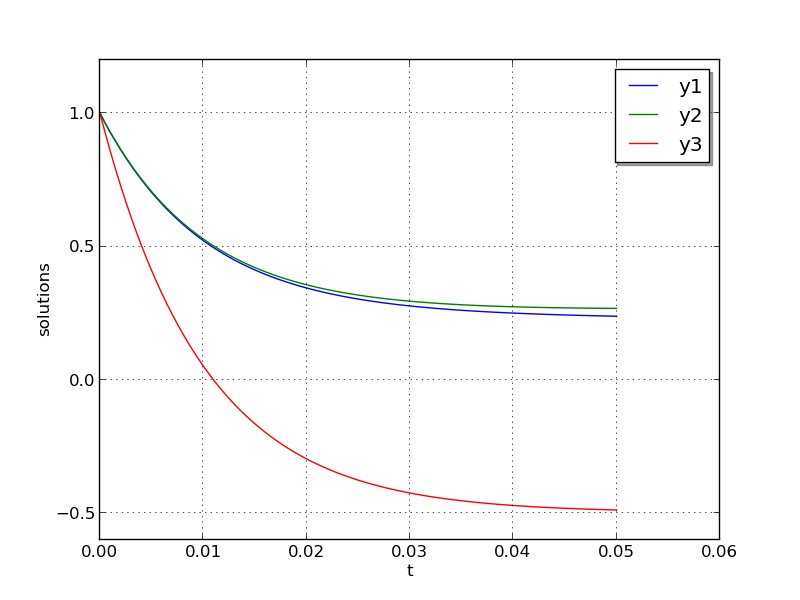
\includegraphics[width=0.450\linewidth]{plot-ark_analytic_sys.png}

\includegraphics[width=0.450\linewidth]{plot-ark_analytic_sys_error.png}


\chapter{Parallel C++ example problems}
\label{cpp_parallel:parallel-cpp}\label{cpp_parallel::doc}\label{cpp_parallel:parallel-c-example-problems}

\section{ark\_heat2D}
\label{cpp_parallel:ark-heat2d}\label{cpp_parallel:id1}
ARKode provides one parallel C++ example problem, that extends our
previous {\hyperref[c_serial:ark-heat1d]{\emph{\DUspan{}{ark\_heat1D}}}} test to now simulate a two-dimensional heat
equation,
\begin{gather}
\begin{split}\frac{\partial u}{\partial t} = k_x \frac{\partial^2 u}{\partial x^2}
                              + k_y \frac{\partial^2 u}{\partial y^2} + h,\end{split}\notag
\end{gather}
for \(t \in [0, 0.3]\), and \((x,y) \in [0, 1]^2\), with initial
condition \(u(0,x,y) = 0\), stationary boundary conditions,
\begin{gather}
\begin{split}\frac{\partial u}{\partial t}(t,0,y) = \frac{\partial u}{\partial t}(t,1,y) =
\frac{\partial u}{\partial t}(t,x,0) = \frac{\partial u}{\partial t}(t,x,1) = 0,\end{split}\notag
\end{gather}
and a periodic heat source,
\begin{gather}
\begin{split}h(x,y) = \sin(\pi x) \sin(2\pi y).\end{split}\notag
\end{gather}
Under these conditions, the problem has an analytical solution of the
form
\begin{gather}
\begin{split}u(t,x,y) = \frac{1 - e^{-(k_x+4k_y)\pi^2 t}}{(k_x+4k_y)\pi^2} \sin(\pi x) sin(2\pi y).\end{split}\notag
\end{gather}

\subsection{Numerical method}
\label{cpp_parallel:numerical-method}
The spatial derivatives are computed using second-order centered
differences, with the data distributed over \(nx\times ny\) points
on a uniform spatial grid.

The problem is set up to use spatial grid parameters \(nx=60\) and
\(ny=120\), with heat conductivity parameters \(k_x=0.5\) and
\(k_y=0.75\).  The problem is run using scalar relative and
absolute solver tolerances of \(rtol=10^{-5}\) and
\(atol=10^{-10}\).

As with the 1D version, this program solves the problem with a DIRK
method, that itself uses a Newton iteration and SUNLINSOL\_PCG
iterative linear solver through the ARKSPILS interface.  However,
unlike the previous example, here the PCG solver is preconditioned
using a single Jacobi iteration, and uses ARKSPILS' built-in
finite-difference Jacobian-vector product routine. Additionally, this
problem uses MPI and the NVECTOR\_PARALLEL module for parallelization.


\subsection{Solutions}
\label{cpp_parallel:solutions}
Top row: 2D heat PDE solution snapshots, the left is at time \(t=0\),
center is at time \(t=0.03\), right is at time \(t=0.3\).
Bottom row, absolute error in these solutions.  Note that the relative
error in these results is on the order \(10^{-4}\), corresponding
to the spatial accuracy of the relatively coarse finite-difference
mesh.  All plots are created using the supplied Python script,
\code{plot\_heat2D.py}.

\includegraphics[width=0.300\linewidth]{plot-ark_heat2d_1.png}

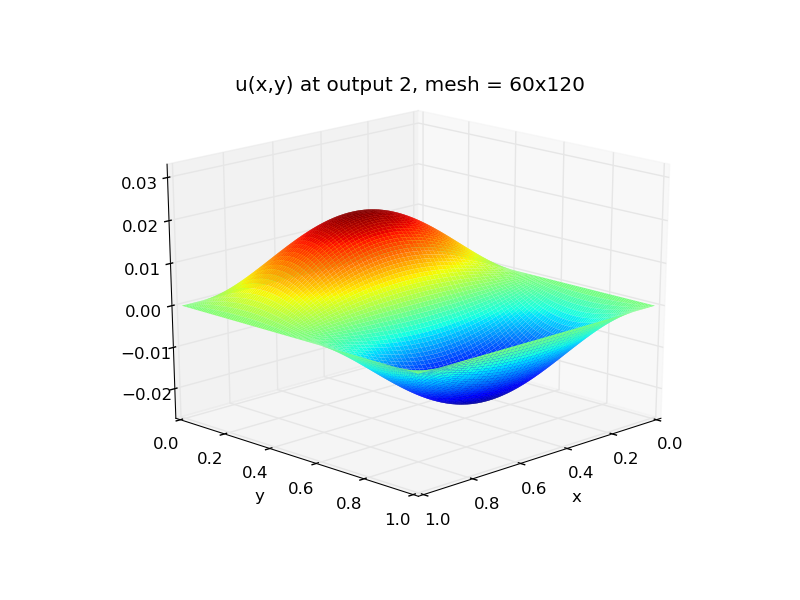
\includegraphics[width=0.300\linewidth]{plot-ark_heat2d_2.png}

\includegraphics[width=0.300\linewidth]{plot-ark_heat2d_3.png}

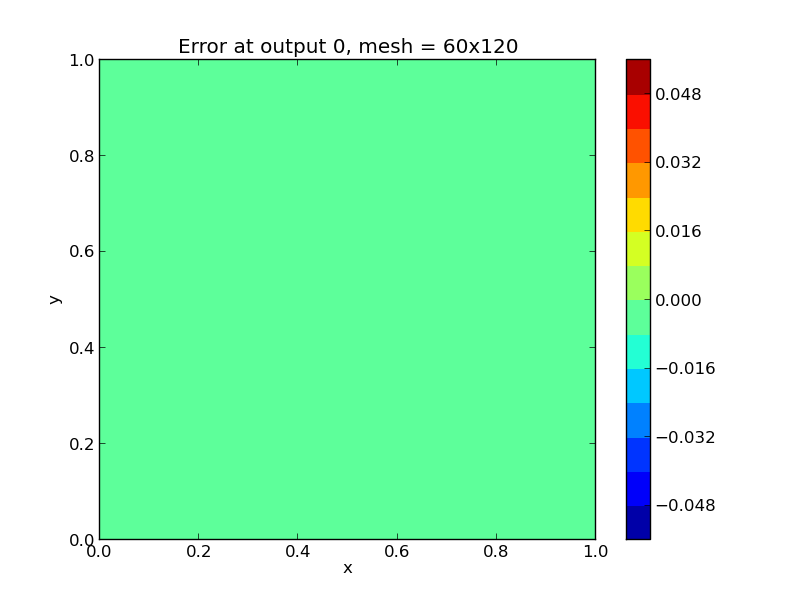
\includegraphics[width=0.300\linewidth]{plot-ark_heat2d_err_1.png}

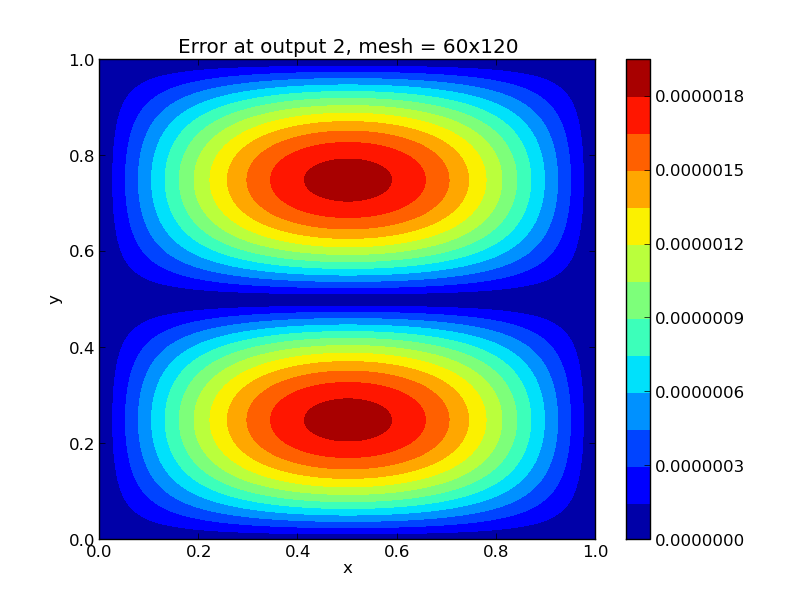
\includegraphics[width=0.300\linewidth]{plot-ark_heat2d_err_2.png}

\includegraphics[width=0.300\linewidth]{plot-ark_heat2d_err_3.png}


\chapter{Serial Fortran 77 example problems}
\label{f77_serial:serial-fortran-77-example-problems}\label{f77_serial::doc}\label{f77_serial:serial-f77}

\section{fark\_diurnal\_kry\_bp}
\label{f77_serial:fark-diurnal-kry-bp}\label{f77_serial:id1}
This problem is an ARKode clone of the CVODE problem,
\code{fcv\_diurnal\_kry\_bp}.  As described in \phantomsection\label{f77_serial:id2}{\hyperref[References:hsr2017]{\emph{{[}HSR2017{]}}}}, this problem
models a two-species diurnal kinetics advection-diffusion PDE system
in two spatial dimensions,
\begin{gather}
\begin{split}\frac{\partial c_i}{\partial t} &=
  K_h \frac{\partial^2 c_i}{\partial x^2} +
  V \frac{\partial     c_i}{\partial x} +
  \frac{\partial}{\partial y}\left( K_v(y)
  \frac{\partial c_i}{\partial y}\right) +
  R_i(c_1,c_2,t),\quad i=1,2\end{split}\notag
\end{gather}
where
\begin{gather}
\begin{split}R_1(c_1,c_2,t) &= -q_1*c_1*c_3 - q_2*c_1*c_2 + 2*q_3(t)*c_3 + q_4(t)*c_2, \\
R_2(c_1,c_2,t) &=  q_1*c_1*c_3 - q_2*c_1*c_2 - q_4(t)*c_2, \\
K_v(y) &= K_{v0} e^{y/5}.\end{split}\notag
\end{gather}
Here \(K_h\), \(V\), \(K_{v0}\), \(q_1\), \(q_2\),
and \(c_3\) are constants, and \(q_3(t)\) and \(q_4(t)\)
vary diurnally.  The problem is posed on the square spatial domain
\((x,y) \in [0,20]\times[30,50]\), with homogeneous Neumann
boundary conditions, and for time interval \(t\in [0,86400]\) sec
(1 day).

We enforce the initial conditions
\begin{gather}
\begin{split}c^1(x,y) &=  10^6 \chi(x)\eta(y) \\
c^2(x,y) &=  10^{12} \chi(x)\eta(y) \\
\chi(x) &= 1 - \sqrt{\frac{x - 10}{10}} + \frac12 \sqrt[4]{\frac{x - 10}{10}} \\
\eta(y) &= 1 - \sqrt{\frac{y - 40}{10}} + \frac12 \sqrt[4]{\frac{x - 10}{10}}.\end{split}\notag
\end{gather}

\subsection{Numerical method}
\label{f77_serial:numerical-method}
We employ a method of lines approach, wherein we first semi-discretize
in space to convert the system of 2 PDEs into a larger system of ODEs.
To this end, the spatial derivatives are computed using second-order
centered differences, with the data distributed over \(Mx*My\)
points on a uniform spatial grid.  As a result, ARKode approaches the
problem as one involving \(2*Mx*My\) coupled ODEs. In this
problem, we use a relatively coarse uniform mesh with
\(Mx=My=10\).

This program solves the problem with a DIRK method, using a Newton
iteration with the preconditioned SUNLINSOL\_SPGMR iterative linear
solver module, and the ARKSPILS interface.

The left preconditioner used is a banded matrix, constructed using
the ARKBP module.  The banded preconditioner matrix is generated using
difference quotients, with half-bandwidths \code{mu = ml = 2}.

Performance data and sampled solution values are printed at
selected output times, and all performance counters are printed
on completion.


\section{fark\_roberts\_dnsL}
\label{f77_serial:fark-roberts-dnsl}\label{f77_serial:id3}
This problem is an ARKode clone of the CVODE problem,
\code{fcv\_roberts\_dnsL}.  As described in \phantomsection\label{f77_serial:id4}{\hyperref[References:hsr2017]{\emph{{[}HSR2017{]}}}}, this problem models
the kinetics of a three-species autocatalytic reaction.  This is an
ODE system with 3 components, \(Y = [y_1,\, y_2,\, y_3]^T\),
satisfying the equations,
\begin{gather}
\begin{split}\frac{d y_1}{dt} &= -0.04 y_1 + 10^4 y_2 y_3, \\
\frac{d y_2}{dt} &= 0.04 y_1 - 10^4 y_2 y_3 - 3\cdot10^7 y_2^2, \\
\frac{d y_3}{dt} &= 3\cdot10^7 y_2^2.\end{split}\notag
\end{gather}
We integrate over the interval \(0\le t\le 4\cdot10^{10}\), with initial
conditions  \(Y(0) = [1,\, 0,\, 0]^T\).

Additionally, we supply the following two root-finding equations:
\begin{gather}
\begin{split}g_1(u) = u - 10^{-4}, \\
g_2(w) = w - 10^{-2}.\end{split}\notag
\end{gather}
While these are not inherently difficult nonlinear equations, they
easily serve the purpose of determining the times at which our
solutions attain desired target values.


\subsection{Numerical method}
\label{f77_serial:id5}
This program solves the problem with a DIRK method, using a Newton
iteration with the SUNLINSOL\_LAPACKDENSE linear solver module and
ARKDLS interface.

As with the {\hyperref[c_serial:ark-robertson-root]{\emph{\DUspan{}{ark\_robertson\_root}}}} problem, we enable ARKode's
rootfinding module to find the times at which either \(u=10^{-4}\)
or \(w=10^{-2}\).

Performance data and solution values are printed at
selected output times, along with additional output at rootfinding
events.  All performance counters are printed on completion.


\chapter{Parallel Fortran 77 example problems}
\label{f77_parallel::doc}\label{f77_parallel:parallel-f77}\label{f77_parallel:parallel-fortran-77-example-problems}

\section{fark\_diag\_kry\_bbd\_p}
\label{f77_parallel:fark-diag-kry-bbd-p}\label{f77_parallel:id1}
This problem is an ARKode clone of the CVODE problem,
\code{fcv\_diag\_kry\_bbd\_p}.  As described in \phantomsection\label{f77_parallel:id2}{\hyperref[References:hsr2017]{\emph{{[}HSR2017{]}}}}, this problem
models a stiff, linear, diagonal ODE system,
\begin{gather}
\begin{split}\frac{\partial y_i}{\partial t} &= -\alpha i y_i, \quad i=1,\ldots N.\end{split}\notag
\end{gather}
Here \(\alpha=10\) and \(N=10 N_P\), where \(N_P\) is the
number of MPI tasks used for the problem.  The problem has initial
conditions \(y_i=1\) and evolves for the time interval \(t\in
[0,1]\).


\subsection{Numerical method}
\label{f77_parallel:numerical-method}
This program solves the problem with a DIRK method, using a Newton
iteration with the preconditioned SUNLINSOL\_SPGMR iterative linear
solver module and ARKSPILS interface.

A diagonal preconditioner matrix is used, formed automatically through
difference quotients within the ARKBBDPRE module.  Since ARKBBDPRE is
developed for use of a block-banded preconditioner, in this solver
each block is set to have half-bandwidths \code{mudq = mldq = 0} to
retain only the diagonal portion.

Two runs are made for this problem, first with left and then with
right preconditioning (\code{IPRE} is first set to 1 and then to 2).

Performance data is printed at selected output times, and maximum
errors and final performance counters are printed on completion.


\section{fark\_diag\_non\_p}
\label{f77_parallel:fark-diag-non-p}\label{f77_parallel:id3}
This problem is an ARKode clone of the CVODE problem,
\code{fcv\_diag\_non\_p}.  As described in \phantomsection\label{f77_parallel:id4}{\hyperref[References:hsr2017]{\emph{{[}HSR2017{]}}}}, this problem models a
nonstiff, linear, diagonal ODE system,
\begin{gather}
\begin{split}\frac{\partial y_i}{\partial t} &= -\alpha i y_i, \quad i=1,\ldots N.\end{split}\notag
\end{gather}
Here \(\alpha=\frac{10}{N}\) and \(N=10 N_P\), where \(N_P\) is the
number of MPI tasks used for the problem.  The problem has initial
conditions \(y_i=1\) and evolves for the time interval \(t\in [0,1]\).


\subsection{Numerical method}
\label{f77_parallel:id5}
This program solves the problem with an ERK method, and hence does not
require either a nonlinear or linear solver for integration.

Performance data is printed at selected output times, and maximum
errors and final performance counters are printed on completion.


\chapter{Serial Fortran 90 example problems}
\label{f90_serial:serial-f90}\label{f90_serial:serial-fortran-90-example-problems}\label{f90_serial::doc}

\section{ark\_bruss}
\label{f90_serial:ark-bruss}\label{f90_serial:id1}
This test problem is a Fortran-90 version of the same brusselator
problem as before, {\hyperref[c_serial:ark-brusselator]{\emph{\DUspan{}{ark\_brusselator}}}}, in which the ``test 1''
parameters are hard-coded into the solver.  As with the previous test,
this problem has 3 dependent variables \(u\), \(v\) and
\(w\), that depend on the independent variable \(t\) via the
IVP system
\begin{gather}
\begin{split}\frac{du}{dt} &= a - (w+1)u + v u^2, \\
\frac{dv}{dt} &= w u - v u^2, \\
\frac{dw}{dt} &= \frac{b-w}{\varepsilon} - w u.\end{split}\notag
\end{gather}
We integrate over the interval \(0 \le t \le 10\), with the
initial conditions \(u(0) = 3.9\), \(v(0) = 1.1\),
\(w(0) = 2.8\), and parameters \(a=1.2\), \(b=2.5\) and
\(\varepsilon=10^{-5}\).  After each unit time interval, the
solution is output to the screen.


\subsection{Numerical method}
\label{f90_serial:numerical-method}
Since this driver and utility functions are written in Fortran-90,
this example demonstrates the use of the FARKODE interface for the
ARKode solver.  For time integration, this example uses the
fourth-order additive Runge-Kutta IMEX method, where the right-hand
sides are broken up as
\begin{gather}
\begin{split}f_E(t,u,v,w) = \left(\begin{array}{c} a - (w+1)u + v u^2 \\
  w u - v u^2 \\ - w u  \end{array}\right), \quad\text{and}\quad
f_I(t,u,v,w) = \left(\begin{array}{c} 0\\0\\
  \frac{b-w}{\varepsilon}\end{array}\right).\end{split}\notag
\end{gather}
The implicit systems are solved using the built-in modified Newton
iteration, with the SUNMATRIX\_DENSE matrix module and accompanying
SUNLINSOL\_DENSE linear solver module, through the ARKDLS interface.
Both the Jacobian routine and right-hand side functions are supplied
by functions provided in the example file.

The only non-default solver options are the tolerances
\(atol=10^{-10}\) and \(rtol=10^{-6}\), adaptivity method 2 (I
controller), a maximum of 8 Newton iterations per step, a nonlinear
solver convergence coefficient \(nlscoef=10^{-8}\), and a maximum
of 1000 internal time steps.


\subsection{Solutions}
\label{f90_serial:solutions}
With this setup, all three solution components exhibit a rapid
transient change during the first 0.2 time units, followed by a slow
and smooth evolution, as seen in the figure below.  Note that these
results identically match those from the previous C example with the
same equations.
\begin{figure}[htbp]
\centering

\scalebox{0.700000}{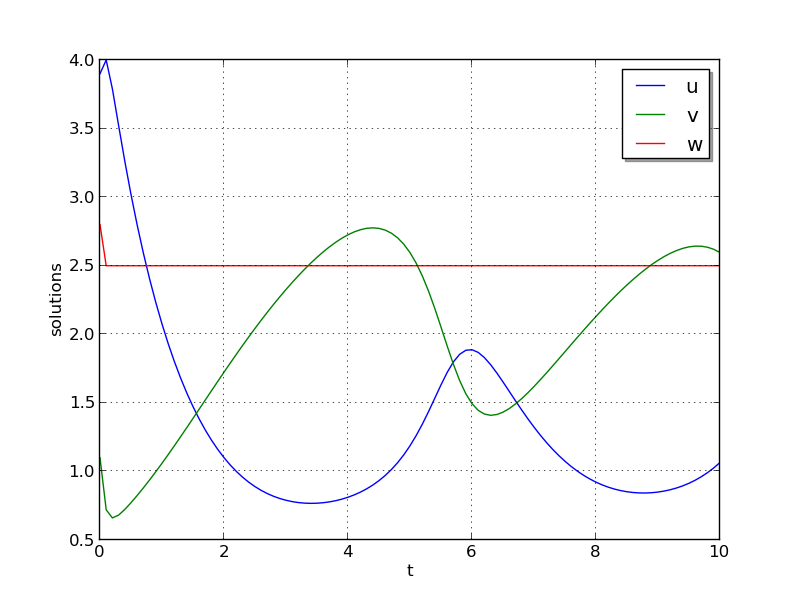
\includegraphics{plot-ark_bruss1.png}}
\end{figure}


\section{ark\_bruss1D\_FEM\_klu}
\label{f90_serial:ark-bruss1d-fem-klu}\label{f90_serial:id2}
This problem is mathematically identical to the C example problem
{\hyperref[c_serial:ark-brusselator1d-fem-slu]{\emph{\DUspan{}{ark\_brusselator1D\_FEM\_slu}}}}, but is written in Fortran 90, stores
the sparse Jacobian and mass matrices in compressed-sparse-row format,
and uses the KLU sparse-direct linear solver.


\chapter{Parallel Fortran 90 example problems}
\label{f90_parallel:parallel-fortran-90-example-problems}\label{f90_parallel::doc}\label{f90_parallel:parallel-f90}

\section{fark\_heat2D}
\label{f90_parallel:fark-heat2d}\label{f90_parallel:id1}
This test problem is a Fortran-90 version of the same two-dimensional
heat equation problem as in C++, {\hyperref[cpp_parallel:ark-heat2d]{\emph{\DUspan{}{ark\_heat2D}}}}.  This models a
simple two-dimenaional heat equation,
\begin{gather}
\begin{split}\frac{\partial u}{\partial t} = k_x \frac{\partial^2 u}{\partial x^2}
                              + k_y \frac{\partial^2 u}{\partial y^2} + h,\end{split}\notag
\end{gather}
for \(t \in [0, 0.3]\), and \((x,y) \in [0, 1]^2\), with initial
condition \(u(0,x,y) = 0\), stationary boundary conditions,
\begin{gather}
\begin{split}\frac{\partial u}{\partial t}(t,0,y) = \frac{\partial u}{\partial t}(t,1,y) =
\frac{\partial u}{\partial t}(t,x,0) = \frac{\partial u}{\partial t}(t,x,1) = 0,\end{split}\notag
\end{gather}
and a periodic heat source,
\begin{gather}
\begin{split}h(x,y) = \sin(\pi x) \sin(2\pi y).\end{split}\notag
\end{gather}
Under these conditions, the problem has an analytical solution of the
form
\begin{gather}
\begin{split}u(t,x,y) = \frac{1 - e^{-(k_x+4k_y)\pi^2 t}}{(k_x+4k_y)\pi^2} \sin(\pi x) sin(2\pi y).\end{split}\notag
\end{gather}

\subsection{Numerical method}
\label{f90_parallel:numerical-method}
The spatial derivatives are computed using second-order centered
differences, with the data distributed over \(nx\times ny\) points
on a uniform spatial grid.

The spatial grid is set to \(nx=60\) and \(ny=120\).  The heat
conductivity parameters are \(k_x=0.5\) and \(k_y=0.75\).

As with the C++ version, this program solves the problem with a DIRK
method, that itself uses a Newton iteration and SUNLINSOL\_PCG
iterative linear solver module through the ARKSPILS interface.  Also
like the C++ version, the PCG solver is preconditioned using a single
Jacobi iteration, and uses ARKSPILS' finite-difference Jacobian-vector
product approximation routine for the PCG polver.  Additionally, this
problem uses MPI and the Fortran interface to the NVECTOR\_PARALLEL
module for parallelization.
\phantomsection\label{References:references}
\begin{thebibliography}{HSR2017}
\bibitem[HSR2017]{HSR2017}{\phantomsection\label{References:hsr2017} 
A.C. Hindmarsh, R. Serban and D.R. Reynolds. Example
Programs for CVODE v3.0.0. Technical Report
UCRL-SM-208110, LLNL, 2017.
}
\bibitem[R2018]{R2018}{\phantomsection\label{References:r2018} 
D.R. Reynolds. User Documentation for ARKode
v3.0.0. Technical Report LLNL-CODE-667205, LLNL, 2018.
}
\end{thebibliography}



\renewcommand{\indexname}{Index}
\printindex
\end{document}
